\chapter{Neutrino Unfolding}
\label{ch:gnns}

Particle physics experiments have finite resolution, limited acceptance, and error-prone reconstruction algorithms.
These limitations mean that the actual physical variable of interest $\x$ and its associated distribution $p_\text{true}(\x)$ are not directly observable.
In data, we only have access to some distorted reconstructed proxy variable $\y$ and its distribution $p_\text{data}(\y)$.
MC generators use theoretical assumptions to approximate $p_\text{gen} \approx p_\text{true}$.
Expensive detector simulations allow us to sample from the conditional distribution $p_\text{sim}(\y|\x)$.
This allows us to form our estimation of the data distribution through the marginalization,
\begin{equation}
    \int p_\text{sim}(\y|\x) p_\text{MC}(\x) \diff\x = p_\text{MC}(\y) \approx p_\text{data}(\y).
\end{equation}
If one has access to the reverse process $p_\text{unfold}(\x|\y)$, then one can use it to \textit{unfold} the data by,
\begin{equation}
    \int p_\text{unfold}(\x|\y) p_\text{data}(\y) \diff\y \approx p_\text{true}(\x),
\end{equation}
yielding a direct approximation for the underlying physical distribution.
Unfolding is useful as it allows a comparison between predicted theory and observed data in a way that is independent of the detector response, ensuring that any observed irregularities are due to physics rather than detector artefacts.
Approximating $p_\text{unfold}(\x|\y)$ however is a difficult and ill-possed task: solutions are not unique, and small changes in $p_\text{data}$ can cause large changes in the predicted $p_\text{true}$.

In this chapter we describe the work done to create deep generative models to approximate $f_\theta(\y) \approx p_\text{unfold}(\x|\y)$.
Specifically, we focus on the problem of unfolding the momentum of the neutrinos in the final state of the event.
This is a specifically challenging setting as neutrinos are not directly observable in data.
Their experimental signature \ptmiss, described in \Cref{sec:MET}, only captures a noisy approximation of the net neutrino momentum in the transverse plane.
In order to yield $p_\text{unfold}(\x|\y)$ a significant amount of domain knowledge is required.

This chapter summarizes the work done in \textcite{NuFlows1} and \textcite{Nu2Flows}, which describes the development of models to unfold the neutrino momentum in simulated \ttbar events with one and two neutrinos in the final state, respectively.

\section{Introduction}

Neutrinos couple solely to the weak nuclear force and do not interact with detector material; they escape collider experiments undetected.
Their presence is inferred from the missing transverse momentum $\ptmiss$, calculated from the momentum imbalance of all visible particles in the plane perpendicular to the beam pipe.
It offers an experimental proxy for the net transverse momentum of all undetected particles.
However, no such proxy exists in the longitudinal direction due to the unknown initial momentum of the colliding partons.
Furthermore, this only constrains the total transverse momentum, and for events producing multiple neutrinos, individual kinematics are under-constrained, leading to a continuum of possible solutions given the data.
While these solutions are possible, they are not equally probable, and the goal of this chapter is to determine this probability distribution.

Analyses in collider physics often involve neutrino production and would benefit from determining the individual kinematics of final-state neutrinos.
A notable example is the study of the top quark, which decays almost instantaneously into a $b$-quark and a $W$ boson in 99.9\% of cases.
Approximately one-third of these $W$ bosons decay leptonically, resulting in a final state that includes a neutrino.
As the heaviest particle in the Standard Model, the top quark has the largest coupling to the Higgs boson.
It plays a unique role in the stability of the electroweak vacuum due to its presence in the quadratic term of the Higgs potential.
Its rapid decay offers a unique opportunity to measure the properties of a bare quark.

Reconstructing the \ttbar system, including top quarks decaying leptonically via a $W$ boson, is crucial for many top quark measurements.
However, the unknown momentum of final-state neutrinos makes it impossible to reconstruct the event entirely.

Our method utilizes a deep generative model to approximate the set of neutrino momenta $\{\p^{\nu_i}\}_{i=1}^N$, given all observable objects in the event and the number of neutrinos $N$.
It is trained on simulated events with known neutrino momenta.
Standard deep learning regression methods collapse the posterior into a point estimate, failing to capture solution diversity or uncertainty.
Therefore, a probabilistic approach that provides the likelihood over a range of viable solutions is necessary.

We use a normalizing flow (NF), detailed in \Cref{sec:flows}.
For this task, the NF requires observed data and two main underlying assumptions or implicit biases: the physical process being studied, ingrained into the flow by the training set's composition, and the assumed number of neutrinos or non-interacting particles, built into the flow's structure.
These assumptions are crucial to constraining the solution space.

We call our method \vvflows, and it is composed of two key networks.
The first is an invertible neural network which learns a bijection between truth neutrino momenta and the latent space, each represented as flattened rank-1 tensors, given a context tensor.
The second is a feature extractor, which learns an expressive context tensor given all the visible objects in the event.
Much of the work throughout these projects involved expanding and testing more sophisticated feature extractors.

\section{Single Neutrino Final State}

The simplest case is when there is only one neutrino in the final state which has three dimensions, and we use the semi-leptonic \ttbar decay as a case study\footnote{The code~\cite{SemileptonicTtbarNeutrino} and datasets~\cite{NuFlowsCode} are publicly available.}.
The final-state of this process contains at least four jets, a lepton, and a single neutrino as shown in \Cref{fig:feynman}.

\begin{figure}[ht]
    \center
    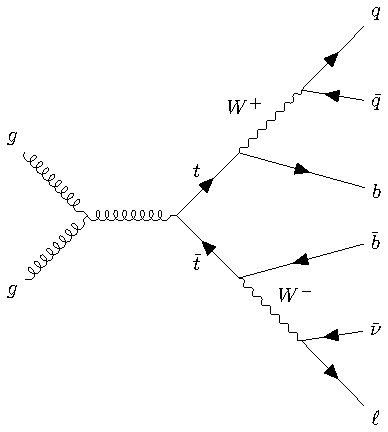
\includegraphics[width=0.4\textwidth]{Figures/neutrino_unfolding/feynman.pdf}
    \caption{A representative Feynman diagram illustrating the semi-leptonic decay of a top quark pair produced the gluon-gluon fusion.}
    \label{fig:feynman}
\end{figure}

\subsection{Quadratic Solution}

For this process, the standard approach~\cite{Quad1, Quad2, Quad4, Quad5} to estimate $\p^\nu$ uses a kinematic constraint,
\begin{equation}
    \label{eq:quadratic}
    p_z^\nu = \frac{-b \pm \sqrt{b^2-4ac}}{2a}, \quad \text{where} \quad
    \begin{aligned}
        \alpha & = m_W^2 - m_\ell^2+2(p_x^\ell p_x^\nu+p_y^\ell p_y^\nu) \\
        a      & = (p_z^\ell)^2 - (E^\ell)^2,                            \\
        b      & = \alpha p_z^\ell,                                      \\
        c      & = \frac{\alpha^2}{4}-(E^\ell)^2(\pt^\nu)^2.
    \end{aligned}
\end{equation}
Here $(p_x^\ell, p_y^\ell, p_z^\ell, E^\ell)$ is the lepton's four-momenta with mass $m_\ell$, and $\pt^\nu$ is the transverse momentum of the neutrino, estimated by $|\ptmiss|$.

This approach has several drawbacks.
It assumes an exact $m_W$, introducing bias by ignoring its natural width.
It also assumes $\pt^\nu$ is perfectly captured by $\ptmiss$, overlooking misidentification and resolution effects.
These factors can result in complex solutions where the convention is to drop the imaginary component.
Additionally, even with perfect reconstruction, the equation will yield two real solutions, with no reason to favour one over the other, though the smaller magnitude result is typically taken.

\subsection{Data}
\label{sec:nu_data}

The data in this study comprises simulated \ttbar events where exactly one top quark decays into a $b$-jet and a leptonically decaying $W^\pm$ boson, resulting in final states with $(e,\nu_e)$, $(\mu,\nu_\mu)$, or their antiparticles.
Around 600k events are used to train the model and an additional 100k events are used for evaluating performance.

\subsubsection{Monte Carlo Generation}

All events are generated from proton-proton collisions at a center-of-mass energy of $\sqrt{s} = 13~\TeV$.
Hard interactions are simulated using \madgraph 3.1.0~\cite{MadGraph}, with decays of top quarks and $W$~bosons modelled with MadSpin~\cite{MadSpin}.
The mass of the top quark is set to $m_t = 173~\GeV$.
Event generation is interfaced to \pythia 8.243~\cite{Pythia8} to model parton shower and hadronisation.
All steps use the \textsc{NNPDF2.3LO} PDF set~\cite{PDF2.3} with $\alpha_S(m_Z) = 0.130$, as provided by the LHAPDF~\cite{LHAPDF6PartonDensity} framework.
The detector response is simulated using \delphes 3.4.2~\cite{Delphes} with a parametrization that mimics the response of the ATLAS detector.
Jets are reconstructed using energy-flow objects and the anti-$k_t$ algorithm~\cite{AntiKt} with a radius parameter of $R = 0.4$ using FastJet~\cite{FastJet}.
Jet $b$-tagging at $\bnom$ is used to identify jets originating from $b$-quarks.

Events are required to contain exactly one reconstructed electron or muon with $p_\mathrm{T} > 15~\GeV$ in the range $|\eta|<2.5$ and at least four jets with $\pt > 25~\GeV$ in the range $|\eta|<2.5$.
At least two of the jets are required to pass the $b$-tagging criteria.
For truth labelling, jets were matched to partons within a radius of $\Delta R < 0.4$.
Events containing jets matched to multiple partons were removed from the training and evaluation datasets.

\subsubsection{Input and Target Features}

Variables from event reconstruction are used as conditioning inputs to the feature extractor network.
Up to 10 jets, as ordered by $p_\mathrm{T}$, are selected per event.
The full set of observed features is described in Table~\ref{tab:inputs}.
The target for the flow is the neutrino three-momentum vector defined by $(p_x^\nu, p_y^\nu, \eta^\nu )$.
The coordinate system used to represent the momentum of each physics object, was optimized as part of a hyperparameter scan.
We found that using $\eta$ instead of $p_z$ and the logarithm of the energy $\log E^j$ yielded the best performance.
We used standard normalization techniques to scale the inputs and targets to zero mean and unit variance.

\begin{table}[ht]
    \caption{The observable inputs used for the event feature extractor.}
    \label{tab:inputs}
    \centering
    \begin{tabular}{r c l}
        \toprule
        Category                & Variables                                              & Description                                 \\
        \midrule
        $\ptmiss$               & $p_x^\text{miss}$, $p_y^\text{miss}$                   & Missing transverse momentum 2-vector        \\ [2ex]
        \multirow{2}{*}{Lepton} & $p_x^{\ell}$, $p_y^{\ell}$, $\eta^\ell$, $\log E^\ell$ & Lepton momentum 4-vector                    \\
                                & $\ell^{flav}$                                          & Whether lepton is an electron or muon       \\ [2ex]
        \multirow{2}{*}{Jets}   & $p_x^{j}$, $p_y^j$, $\eta^j$,  $\log E^j$              & Jet momentum 4-vector                       \\
                                & $isB$                                                  & Whether jet passes $b$-tagging criteria     \\ [2ex]
        Misc                    & $N_{\text{jets}}$, $N_{\text{bjets}}$                  & Jet and $b$-jet multiplicities in the event \\
        \bottomrule
    \end{tabular}
\end{table}

\subsection{Model Architecture}

The \vflows architecture optimized for this process is depicted in \Cref{fig:flow}.
All observed inputs are passed through a feature extractor network to produce a context tensor for the flow.
As there are a variable number of jets in each event, they are first passed through a multi-headed conditional deep set network.
Inside the deep set there are three separate MLPs, one to extract the features, one to calculate the attention weights, and a final network to apply to the aggregated attributes.
The NF was constructed from of seven rational-quadratic spline coupling layers~\cite{NeuralSplineFlows} interleaved with LU-parameterized linear layers.
The latent distribution was chosen to be $\mathcal{N}(0, I)$.

\begin{figure}[ht]
    \centering
    \adjustbox{valign=c}{
        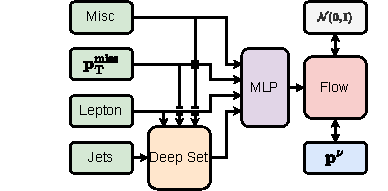
\includegraphics[width=0.49\textwidth]{Figures/neutrino_unfolding/nuflow.pdf}
    }
    \adjustbox{valign=c}{
        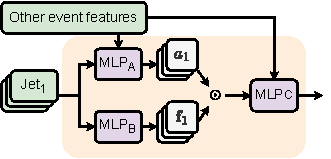
\includegraphics[width=0.3\textwidth]{Figures/neutrino_unfolding/deepset.pdf}
    }
    \caption{The architecture of the \vflows model for the single neutrino case (left), and the attention weighted deep set used in the feature extractor (right).}
    \label{fig:flow}
\end{figure}

The model was constructed using the nflows library~\cite{nflows} and trained using the standard negative log-likelihood loss function.
A cosine annealing scheduler adjusted the learning rate from zero to $5\times 10^{-4}$ every two epochs.
Gradient clipping with a max-norm of 5 ensured stable convergence.
For cross-validation, $10\%$ of the training data was reserved as a holdout set, and early-stopping was applied using a 30-epoch patience parameter.
We used the Adam optimizer~\cite{Adam} with default parameters and a 256 batch size.
The training was done on an NVIDIA 2080-Ti GPU, with the NF taking around 4 hours to converge.

To compare performance with standard regression, we also trained a feed-forward network (FF) using only the feature extractor to predict the neutrino three-momentum directly.
The FF network was trained using Smooth-L1 loss function~\cite{SmoothL1}.
All other training parameters were kept the same.
This approach is termed \vff.

\subsection{Results}

For unfolding, we sample under the flow in reverse-mode, and we call this method \vsample.
This method has low bias but high variance.
Alternatively, we can approximate $\argmax_\X{p_X(\x|\con)}$ by generating 256 neutrinos per event and selecting the solution with the highest likelihood.
We call this method \vmode.
We compare these methods to the mass constraint solution and \vff.
Furthermore, we include reconstruction using the true neutrino momenta; plots labelled \emph{Truth} refer only to the neutrino values, while other properties, such as those of leptons or jets, are from reconstructed objects.

\subsubsection{Per Event Inference}

\Cref{fig:inference} illustrates the benefits of \vflows by comparing the reconstruction methods in $\eta^\nu$ for three samples.
In \Cref{fig:inf_good} the $m_W$ constraint method yields two solutions and there is no indication \textit{a priori} which of these will be closer to the true value.
In contrast, \vflows provides the entire probability distribution across $\eta^\nu$ values, showing two peaks corresponding to the quadratic solutions indicating that it has relearned this kinematic relationship from data.
It also highlights a preference for the solution closer to the actual value.
The \vff yields a point estimate falling between the two peaks, collapsing to the mean of the data distribution due to the symmetrical loss function.
In \Cref{fig:inf_ambig}, \vflows reproduces the multimodal distribution with less preference for either solution.
\Cref{fig:inf_bad} shows an event where no method provides a reasonable estimate for $\eta^\nu$, suggesting poor object reconstruction in the event, particularly \ptmiss.
The increased uncertainty in the likelihood plot of \vflows highlights its ability to identify poorly reconstructed events for filtering as one can devise a method to reject events matching \Cref{fig:inf_bad} and \Cref{fig:inf_ambig}.

\begin{figure}[ht]
    \centering
    \begin{subfigure}{0.32\textwidth}
        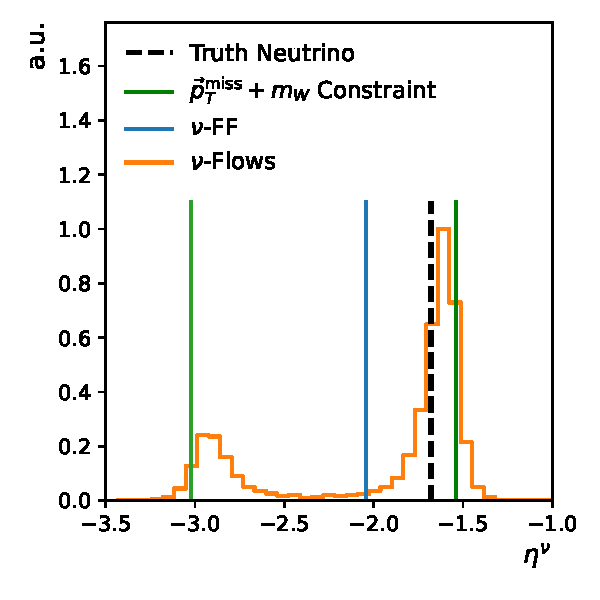
\includegraphics[width=\textwidth]{Figures/neutrino_unfolding/eta_5.pdf}
        \caption{} \label{fig:inf_good}
    \end{subfigure}
    \begin{subfigure}{0.32\textwidth}
        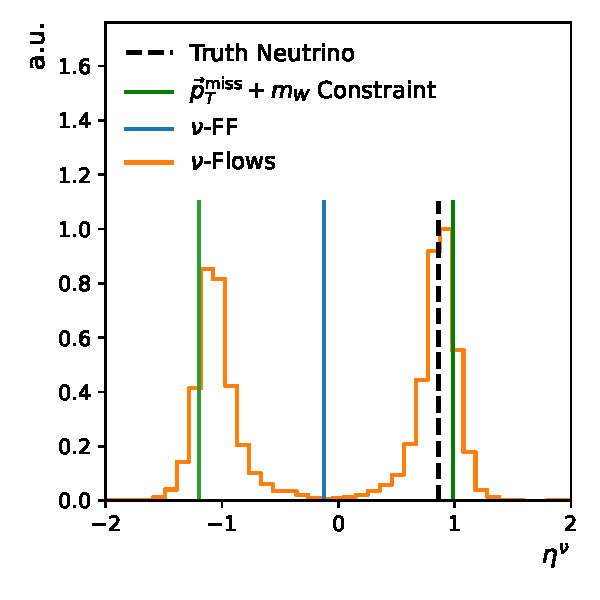
\includegraphics[width=\textwidth]{Figures/neutrino_unfolding/eta_9.pdf}
        \caption{} \label{fig:inf_ambig}
    \end{subfigure}
    \begin{subfigure}{0.32\textwidth}
        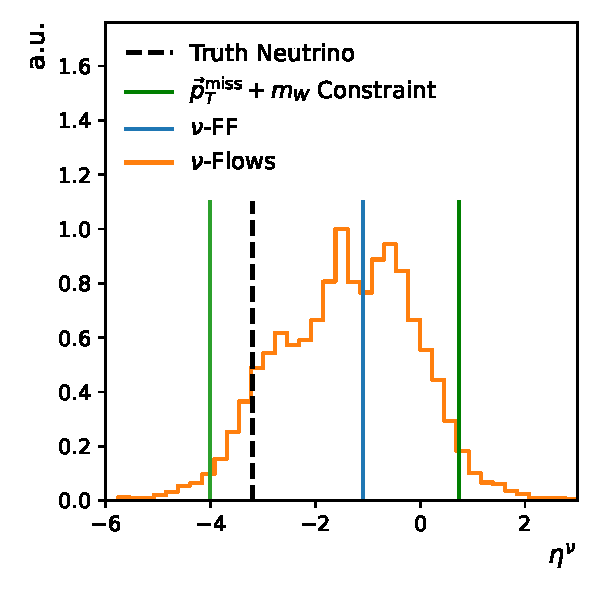
\includegraphics[width=\textwidth]{Figures/neutrino_unfolding/eta_12.pdf}
        \caption{} \label{fig:inf_bad}
    \end{subfigure}
    \caption{The $\eta$ of three different neutrinos selected from the evaluation dataset. The true values are shown in black. The two solutions from the $m_W$ constraint method are shown in green. The single point estimate using \vff is shown in blue. The probability density learned by \vflows is shown in orange.}
    \label{fig:inference}
\end{figure}

\subsubsection{Momentum Distributions}

The marginal distributions of $p_z^\nu$ and $E^\nu$ are shown in \Cref{fig:marginal_dists}.
Both the quadratic mass constraint and \vff methods exhibit a bias towards zero in $p_z^\nu$.
This also results in a bias towards lower $E^\nu$ values which is not present in \vsample.
However, these plots could be constructed with non-conditional generative models, and the real power of \vflows is in the joint distributions.
\Cref{fig:dists} shows 2D histograms of reconstructed and true $p_z^\nu$ coordinates, highlighting the zero bias in \vff and $m_W$ constraint methods.
Both \vflows models correlate well with the true values, although \vsample exhibits higher variance.

\begin{figure}[ht]
    \centering
    \begin{subfigure}{0.40\textwidth}
        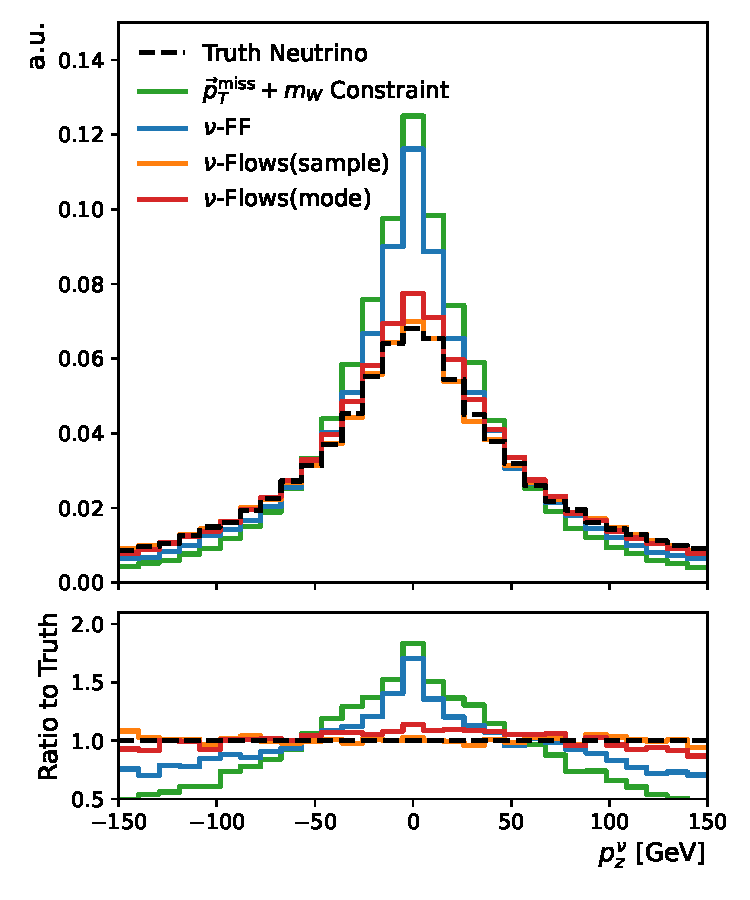
\includegraphics[width=\textwidth]{Figures/neutrino_unfolding/p_z.pdf}
        \caption{} \label{fig:nu_pz}
    \end{subfigure}
    \begin{subfigure}{0.40\textwidth}
        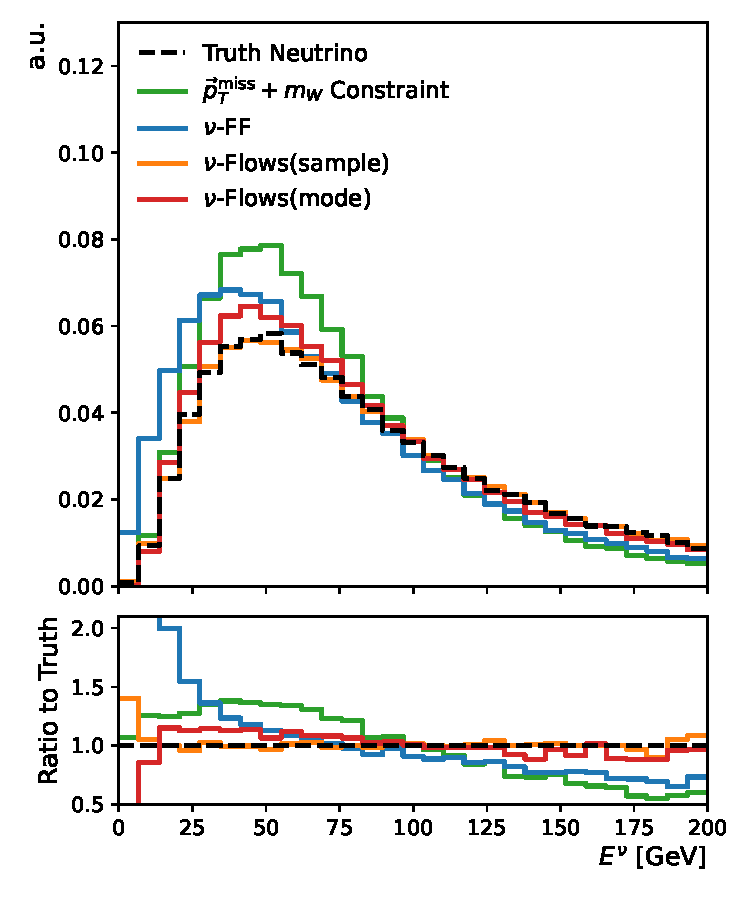
\includegraphics[width=\textwidth]{Figures/neutrino_unfolding/E.pdf}
        \caption{} \label{fig:nu_E}
    \end{subfigure}
    \caption{Distributions of the reconstructed $p_z^\nu$ \subref{fig:nu_pz} and $E^\nu$ \subref{fig:nu_E} using different neutrino reconstruction methods.}
    \label{fig:marginal_dists}
\end{figure}


\begin{figure}[ht]
    \centering
    \begin{subfigure}{0.40\textwidth}
        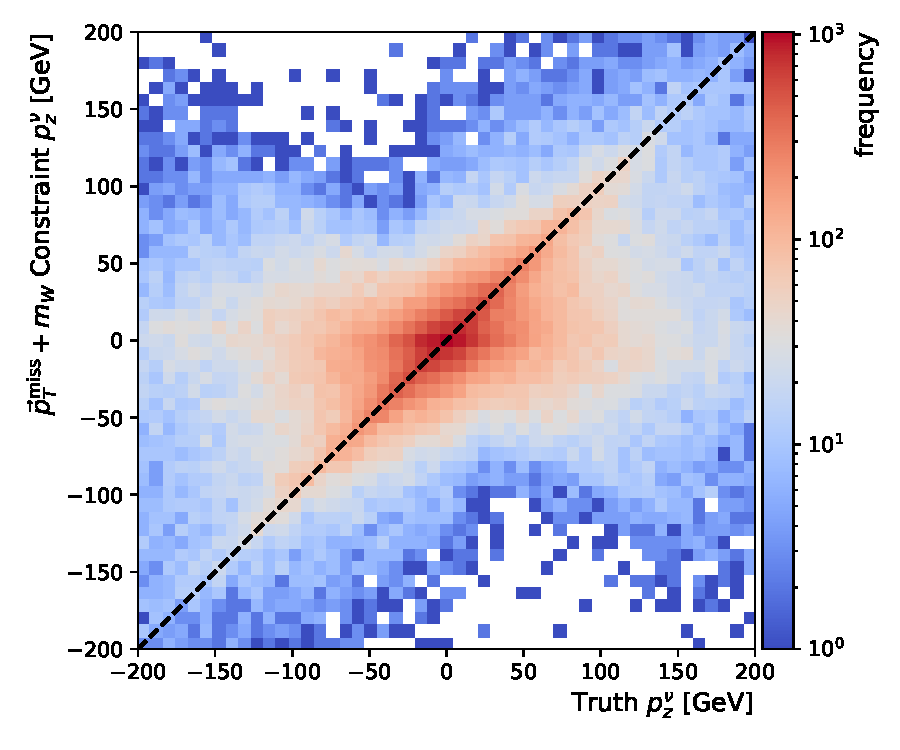
\includegraphics[width=\textwidth]{Figures/neutrino_unfolding/p_z_quad.pdf}
        \caption{} \label{fig:px_dist}
    \end{subfigure}
    \begin{subfigure}{0.40\textwidth}
        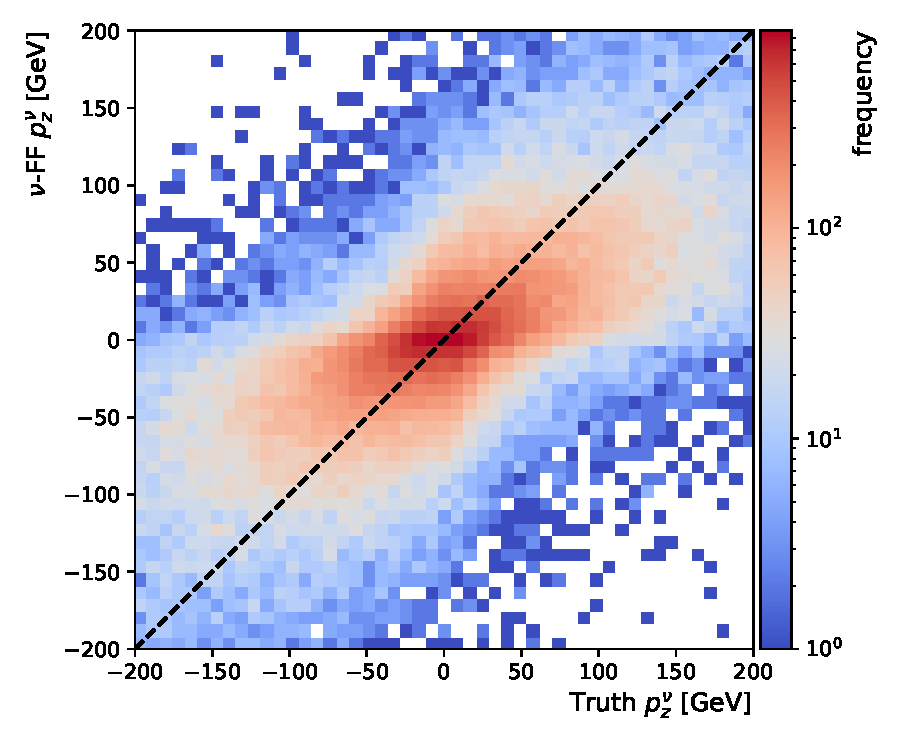
\includegraphics[width=\textwidth]{Figures/neutrino_unfolding/p_z_ff.pdf}
        \caption{} \label{fig:py_dist}
    \end{subfigure}\\
    \begin{subfigure}{0.40\textwidth}
        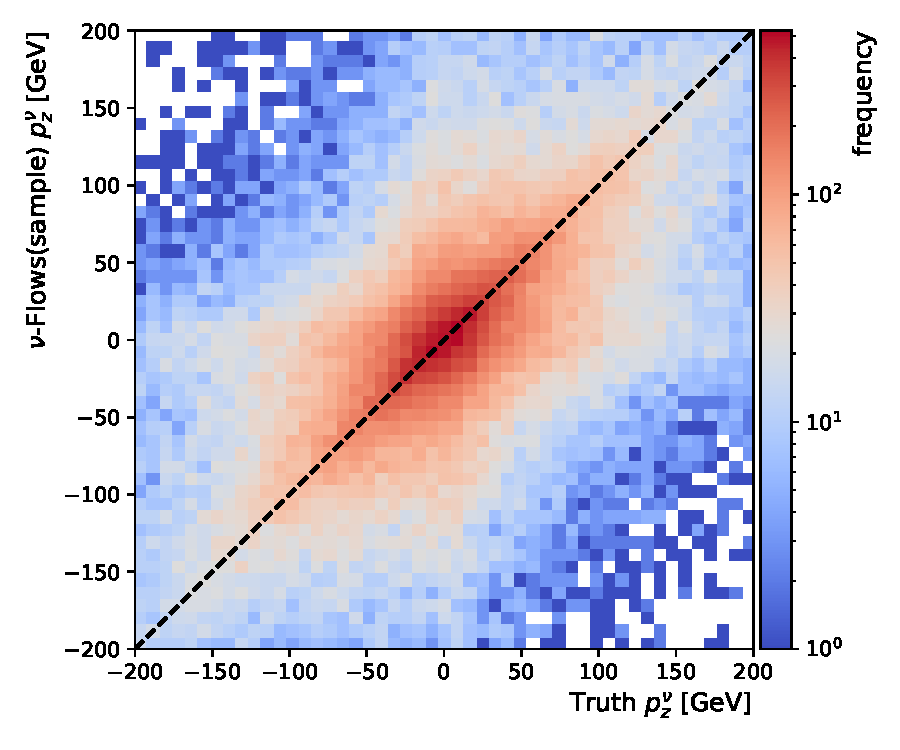
\includegraphics[width=\textwidth]{Figures/neutrino_unfolding/p_z_sample.pdf}
        \caption{} \label{fig:pz_dist}
    \end{subfigure}
    \begin{subfigure}{0.40\textwidth}
        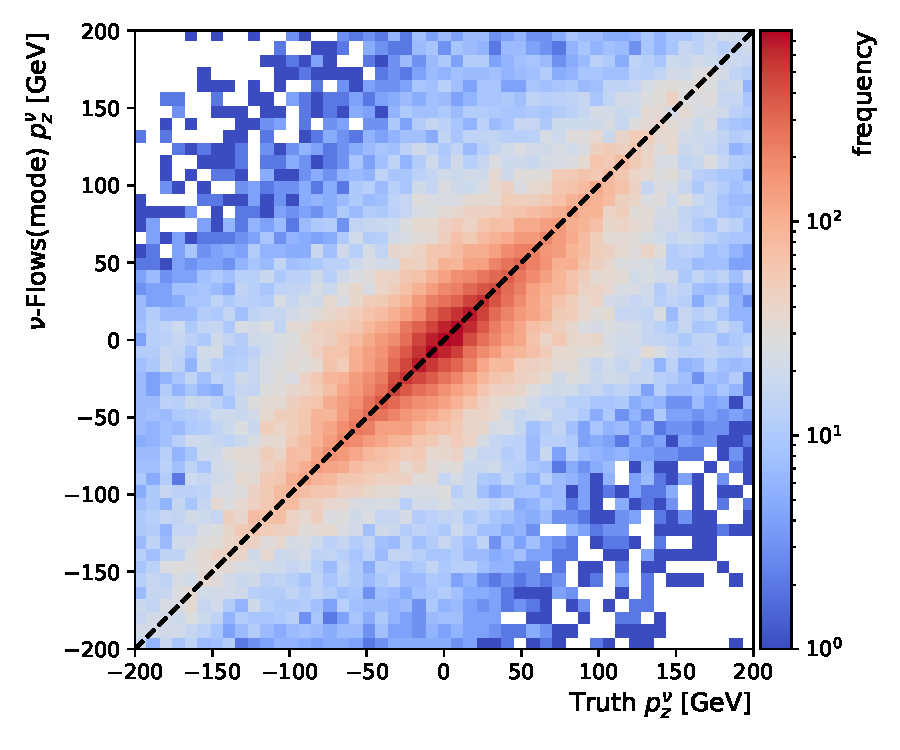
\includegraphics[width=\textwidth]{Figures/neutrino_unfolding/p_z_mode.pdf}
        \caption{} \label{fig:E_dist}
    \end{subfigure}
    \caption{Two-dimensional histograms showing the reconstructed versus true $p_z^\nu$ using the $m_W$ constraint \subref{fig:px_dist}, \vff \subref{fig:py_dist}, \vsample \subref{fig:pz_dist}, and \vmode \subref{fig:E_dist} methods.}
    \label{fig:dists}
\end{figure}

\Cref{fig:lv_mass} shows the reconstructed invariant mass of the leptonic $W$, calculated using the reconstructed lepton and each neutrino estimate.
\vsample nearly matches the true neutrino distribution, while \vmode is centred around the mean.
\vff shows a notable offset of the mean by around $6~\GeV$.
The $m_W$ constraint yields $m_{\ell\nu} = 80.38~\GeV$ for nearly all events, with a positive tail due to no real solutions for the quadratic equation.
The reconstructed invariant mass of the leptonic top quark is shown in \Cref{fig:blv_mass} using the correct $b$-jet from the leptonically decaying top quark to highlight the neutrino reconstruction effect.
Each method shows an increase invariance and a negative bias in the reconstructed mass.
The distribution closest to truth is \vsample.

\begin{figure}[htp]
    \centering
    \begin{subfigure}{0.40\textwidth}
        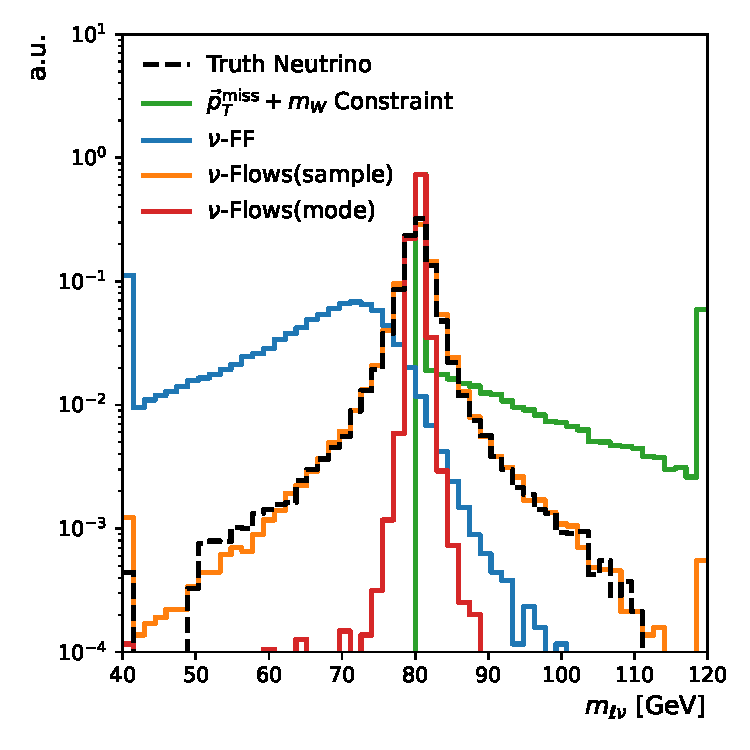
\includegraphics[width=\textwidth]{Figures/neutrino_unfolding/lnu_mass.pdf}
        \caption{} \label{fig:lv_mass}
    \end{subfigure}
    \begin{subfigure}{0.40\textwidth}
        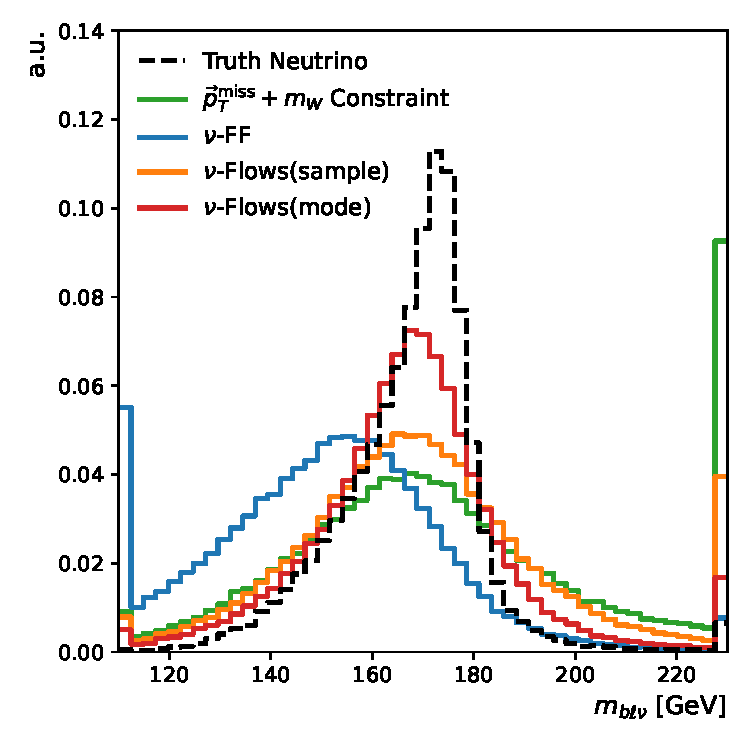
\includegraphics[width=\textwidth]{Figures/neutrino_unfolding/blnu_mass.pdf}
        \caption{} \label{fig:blv_mass}
    \end{subfigure}
    \caption{Distributions of the invariant mass of the $\ell\nu$ \subref{fig:lv_mass} and $b\ell\nu$ \subref{fig:blv_mass} systems using different neutrino reconstruction methods. All methods use reconstructed variables for the lepton and jet kinematics.}
    \label{fig:real_assoc_masses}
\end{figure}

\subsubsection{Jet Association}

We examine the effect of \vflows on the combinatoric assignment of jets to final-state partons.
This task is crucial for top quark physics analyses such as measurements of the top quark mass~\cite{ATLAS:2015pfy,CMS:2018quc,ATLAS:2018fwq,ATLAS:2019guf}, differential cross-sections~\cite{CMS:2016oae,CMS:2018htd,Quad4,CMS:2021vhb}, spin correlation~\cite{CMS:2015cal} and charge asymmetry~\cite{ATLAS:2022waa}.

Semi-leptonic \ttbar events feature four final state partons: $b_{lep}$, $b_{had}$, and the hadronically decaying $W$ boson products, $q_1$ and $q_2$.
These objects may be reconstructed as jets, but so too are signals from initial-state radiation and final-state radiation.
Jet assignment often utilizes a $\chi^2$ fit~\cite{Chi2ATLAS}, which is dependent on the neutrino kinematics, underscoring the value of precise neutrino estimation.
This fitting procedure is just one of many jet combinatoric solving methods.
Other methods include KLFitter~\cite{KLFitter} or any of the new deep learning approached~\cite{SAJA, SPANet, Spatter, TopoGraphs}.
All of these techniques could also be complemented by \vflows.

In the $\chi^2$ fit method, every possible jet-parton assignment is tested, and the one with the lowest $\chi^2$ value defined by
\begin{equation}
    \chi^2=\frac{(m_W-m_{\ell\nu})^2}{\sigma_{\ell\nu}} +\frac{(m_W-m_{qq})^2}{\sigma_{qq}} +\frac{(m_t-m_{b\ell\nu})^2}{\sigma_{b\ell\nu}} +\frac{(m_t-m_{bqq})^2}{\sigma_{bqq}}
    \label{eq:chi_square}
\end{equation}
is kept.
The $\sigma$ values are derived the root-mean-square error of the relevant mass distributions using the true jet-assignments and each neutrino reconstruction method separately.

We perform the fit using permutations of leading 9 jets in $\pt$ and record the parton association accuracy for each neutrino reconstruction method.
The results are shown in \Cref{tab:blep_1sig}.
The $b_\text{lep}$ matching efficiency heavily depends on the neutrino in the $\chi^2$ fit.
Estimates from either \vsample or \vmode enhance matching efficiency over standard kinematic methods.
Replacing the $m_W$ constraint with \vmode in the $\chi^2$ fit improved accuracy by factors of 1.03 for four-jet events and 1.41 for nine-jet events.
For events with fewer jets, the limited permutations reduce the impact of the neutrino term in Equation~\ref{eq:chi_square}.
Consequently, the relationship between the performance gains of $\nu$-Flows and the jet count is anticipated.
Enhancing jet-parton matching efficiency benefits \ttbar event measurements, and $\nu$-Flows is expected to improve various measurements, although further studies are required to validate these outcomes.

\begin{table}[h]
    \caption{The fraction of events for which the $\chi^2$ method identified the correct $b_{lep}$ jet using the various neutrino estimation methods. The results are binned by the number of reconstructed jets in the event. Events must first pass a selection requirement where the partons were reconstructed as jets, so a correct permutation was at least possible.
        This selection did not change the ranking of the methods.}
    \label{tab:blep_4sig}
    \centering
    \begin{tabular}{l r r r r r r}
        \toprule
                                       & \multicolumn{6}{c}{Number of Jets In Event}                                                                                                \\
        Neutrino Type                  & 4                                           & 5                & 6                & 7                & 8                & 9                \\
        \midrule
        Truth Neutrino                 & 0.864                                       & 0.753            & 0.686            & 0.641            & 0.611            & 0.587            \\
        \midrule
        $\ptmiss$ and $m_W$ Constraint & 0.790                                       & 0.576            & 0.476            & 0.398            & 0.366            & 0.286            \\
        \vff                           & 0.754                                       & 0.533            & 0.410            & 0.353            & 0.300            & 0.302            \\
        \vsample                       & 0.803                                       & 0.624            & 0.515            & 0.457            & 0.391            & 0.357            \\
        \vmode                         & $\mathbf{0.813}$                            & $\mathbf{0.664}$ & $\mathbf{0.575}$ & $\mathbf{0.508}$ & $\mathbf{0.481}$ & $\mathbf{0.405}$ \\
        \bottomrule
    \end{tabular}
\end{table}

\FloatBarrier

\section{Two Neutrino Final State}

The case of two neutrinos in the final state is more challenging as the problem is under-constrained.
In single-neutrino scenarios, the main challenge is recovering the neutrino's longitudinal momentum.
In multi-neutrino events, the complexity increases due to the need to distribute the total missing transverse momentum among all final-state neutrinos.
For this case, we use the dileptonic \ttbar process\footnote{The code~\cite{DileptonicTtbarNeutrino} and datasets~\cite{Nu2FlowsCode} are publicly available.}, which is similar to the semi-leptonic case but with both top quarks decaying leptonically, resulting in final states with two lepton-neutrino pairs.
In each event, there will be one neutrino and one anti-neutrino, giving us the order to define the combined 6-dimensional tensor for the flow.
We label model adapted for this final state as \vvflows.

\subsection{Reference Methods}

Several analytical techniques have been developed to reconstruct the two neutrinos in dilepton \ttbar events, including \emph{Neutrino weighting}~\cite{NuW} (\vweight), an algebraic solution~\cite{AlgebraicApproachSolve}, and the \emph{Ellipse} method~\cite{EllipseMethod}.
These methods have been successfully applied in numerous measurements at the Tevatron and LHC with \vweight being particularly popular.
This study compares \vvflows with \vweight due to its widespread use and the \ellipse method for its computational efficiency.

\subsubsection{Neutrino Weighting}

In \vweight, individual neutrino kinematics are derived from a grid search over possible neutrino rapidities.
Following the procedure defined in Ref.~\cite{ATLAS:2019zrq}, we perform a grid search of $\eta^\nu$ and $\eta^{\bar\nu}$ from -5 to 5 with a step size of 0.2.
For each pair of $\eta$ values, we then iterate through all possible assignments of $b$-tagged jets to the $b$-quarks from the \ttbar decay.
Next, we calculate the neutrino four-momenta using the mass constraints,
\begin{gather}
    \label{eq:mass_constraints}
    (\ell_{1, 2} + \nu_{1, 2})^2 = m_w^2 = 80.38~\GeV^2, \\
    (\ell_{1, 2} + \nu_{1, 2} + b_{1, 2})^2 = m_t^2 = 172.5~\GeV^2,
\end{gather}
where $\ell_{1, 2}$, $\nu_{1, 2}$, and $b_{1, 2}$ represent the four-momenta of the charged leptons, neutrinos, and $b$-tagged jets.
This yields two possible neutrino kinematic solutions.
For each solution, we calculate its weight by comparing the total neutrino transverse momentum \ptvv to the measured \ptmiss,
\begin{equation}
    \label{eq:neutrino_weight}
    w = \exp \left( - \frac{||\ptmiss - \ptvv||_2^2}{2 \sigma^2} \right),
\end{equation}
where $\sigma$ is a fixed resolution scale related to \ptmiss reconstruction.
The $\eta$ pair maximizing $w$ is chosen as the correct solution however any solution which results in a reconstructed $\mttbar < 300~\GeV$ or where either of the two reconstructed top quarks has negative energy automatically rejected.
This represents a very costly computation scan that considers only discrete $\eta$ values.

A notable limitation of this method is that, despite numerous neutrino solutions being tested, constraint systems may still be unsolvable due to measurement errors, incorrect object assignment, or deviations in the masses of the top quarks or
$W$ bosons.
We therefore also iterate over different values of $\mtop$ from 171 to $174~\GeV$ in step sizes of $0.5~\GeV$, which increases the number of hypotheses to test but improves solution efficiency.
We find that approximately 5\% of the time, the \vweight method fails to find a valid solution.

\subsubsection{Ellipse method}

The \ellipse method employs a geometric approach to analytically constrain neutrino kinematics in processes where top quarks decay into leptons and neutrinos~\cite{ellipse}.
For a single neutrino, its momentum is determined using the 4-momenta of the $b$-quark and the charged lepton, the \Wboson mass, and the top quark mass, defining an elliptical surface in the momentum space.
Combining this with observed \ptmiss collapses the solution set to a unique value. For events with two neutrinos, the method is extended to calculate the most probable neutrino pair solutions producing the observed \ptmiss.

We utilize the implementation by the method's authors~\cite{EllipseCode}.
The method's drawbacks include the necessity for precise lepton to $b$-jet matching as well as making hard assumptions on the \Wboson and top quark masses.
Like \vweight, it may yield no solutions.
We use simple $\Delta R$ matching to make the lepton to $b$-jet association, considering only the two leading jets in passing $b$-tagging criteria.
If this assignment fails to yeild a neutrino solution, the opposite association is tested.
We find that the method fails to make an assigment in 22\% of \ttbar dilepton events, more than \vweight, but it requires significantly fewer computational.

\subsection{Data}

In this work, \vvflows is applied to simulated \ttbar events where both top quarks decay leptonically, resulting in a final state with exactly two leptons, two neutrinos and two jets initiated by $b$-hadrons ($b$-jets).
Additional jets arise from ISR and FSR.

All events are simulated in proton-proton collisions at a centre-of-mass energy of \mbox{$\sqrt{s}=13$~TeV}.
Two different samples are generated, each using a different generator for the hard interactions in the matrix element.
In the nominal sample, simulation setting match exactly the description in \Cref{sec:nu_data}.
In the alternative sample, both the hard interactions and parton shower are simulated with \pythia 8.307 with the Monash tuned set of parameters~\cite{Monash} at leading order accuracy.
The same PDF set is used as for the nominal sample.
Detector response, reconstruction, and jet tagging matches the configurations from the the single neutrino case.
Truth association of the lepton to the parent top quark is performed assuming there is no charge misidentification, and the true neutrino momenta are taken directly from simulation.

In total there are 1.02 million events in the nominal sample and 1.4 million events in the alternative sample passing all selection requirements.
940,000 (970,000) events from the nominal (alternative) sample are used to train the network, with 80,000 nominal samples used for evaluation.

The input and target features are nearly the same as in the single neutrino case.
There is the addition of a second lepton and neutrino, and the longitudinal component of all objects is represented with \pz instead of $\eta$.

\subsection{Model Architecture}

The feature extraction network attempts to produce a contextual vector specific to each event to guide the transformations within the normalizing flow.
A significant amount of optimization was performed to find the best architecture compared to the single neutrino case.
To extend the model to handle multiple input leptons, we require a permutation invariant architecture that can accommodate a variable number of inputs, motivating the move to transformers, detailed in \Cref{sec:transformers}.

A schematic of the new \vvflows architecture is shown in \Cref{fig:nunuflows}.
This new model uses object-specific embedding networks to project each input into a common high-dimensional space.
These embeddings are then passed through multiple TE Blocks,
A single global vector is obtained via repeated cross-attention with a learnable class token, following techniques used in vision transformers~\cite{GoingDeeper}.

The specific model used in this section comprises three TE and two CA blocks, each with embedding dimensions of 128 and 4 attention heads.
All embedding MLPs have a single hidden layer of 256 neurons, using LeakyReLU activation and Layer-Normal1ization.
The NF uses ten rational-quadratic spline coupling layers interspersed with LU-parameterized linear layers.
For this model, we switch to the normflows library~\cite{Stimper2023}.
The entire \vvflows model has approximately 600,000 trainable parameters.

We train for 100 epochs using the AdamW~\cite{AdamW} with a weight decay strength of \num{e-4} and a learning rate cycled from \num{e-8} to \num{e-3} every 25 epochs

\begin{figure}[ht]
    \centering
    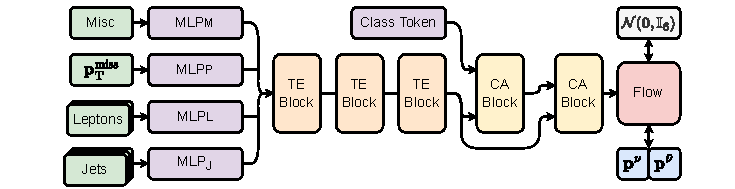
\includegraphics[width=0.99\textwidth]{Figures/neutrino_unfolding/nu2flow.pdf}
    \caption{The architecture of the \vvflows model for the two-neutrino case.}
    \label{fig:nunuflows}
\end{figure}

\subsection{Results}

We compare the performance of the \vvflows model with the \vweight and \ellipse methods.
Also included are results using \vtruth, which uses the true neutrino momenta to establish the performance upper limit for any neutrino reconstruction method.
Note that for \vtruth, all other measurements, like the combined invariant masses, include reconstructed objects.
Using the \textit{mode} method does not improve performance for \vvflows, so all flow results are from sampling under the learned conditional distribution.

A significant drawback of \vweight, leading to the preference for \ellipse despite its reduced performance, is its high computational resource requirement. Conversely, \vflows requires only a single forward pass per event. On a CPU, typical inference times for a single event are around 70 ms, decreasing substantially with parallelized execution on a GPU, as summarized in \Cref{tab:inf_times}.

\begin{table}[htbp]
    \centering
    \caption{Required time for single event inference using \vvflows. Times representative of using a single core of an AMD EPYC 7742 2.25GHz CPU and an NVIDIA 3080 graphics card.}
    \label{tab:inf_times}
    \begin{tabular}{c c c}
        \toprule
        Resource             & Batch size & Time/event [ms] \\
        \midrule
        CPU                  & 1          & 71.4            \\
        \multirow{2}{*}{GPU} & 1          & 33.3            \\
                             & 1000       & 0.03            \\
        \bottomrule
    \end{tabular}
\end{table}

\subsubsection{Kinematic Reconstruction}

The individual neutrino kinematics and the angular separation between the two neutrinos are depicted in \Cref{fig:vvbarkinematics, fig:vreco_delta}.
Both \vweight and \ellipse methods overestimate the neutrino transverse momenta and energy.
These methods also tend to predict neutrino pairs which are back-to-back in $\phi$, with opening angles differing significantly from the ground truth.
In contrast, \vvflows accurately reproduces the ground truth in all neutrino kinematic distributions, with only minor discrepancies in the low-statistic tails.

\begin{figure}[htpb]
    \centering
    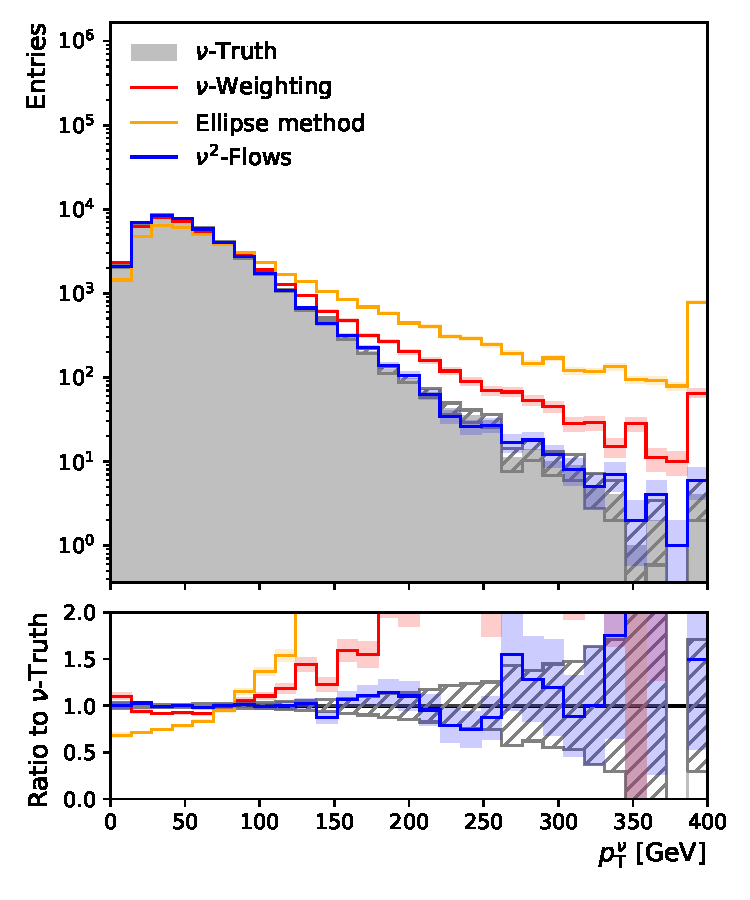
\includegraphics[width=0.32\textwidth]{Figures/neutrino_unfolding/nu_reco/nuanti_nu_pt.pdf}
    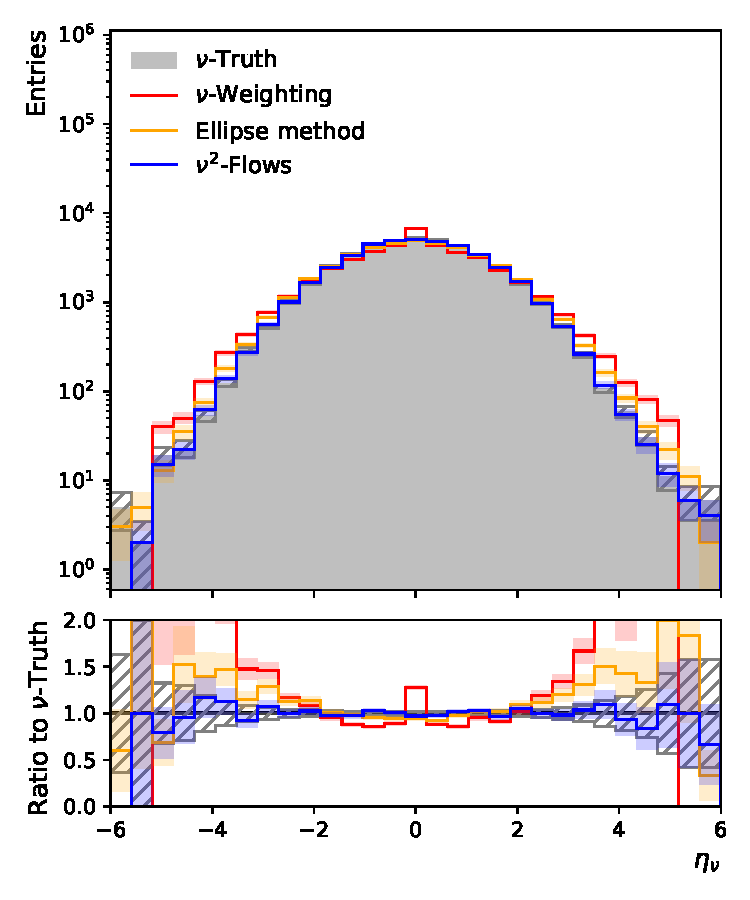
\includegraphics[width=0.32\textwidth]{Figures/neutrino_unfolding/nu_reco/nuanti_nu_eta.pdf}
    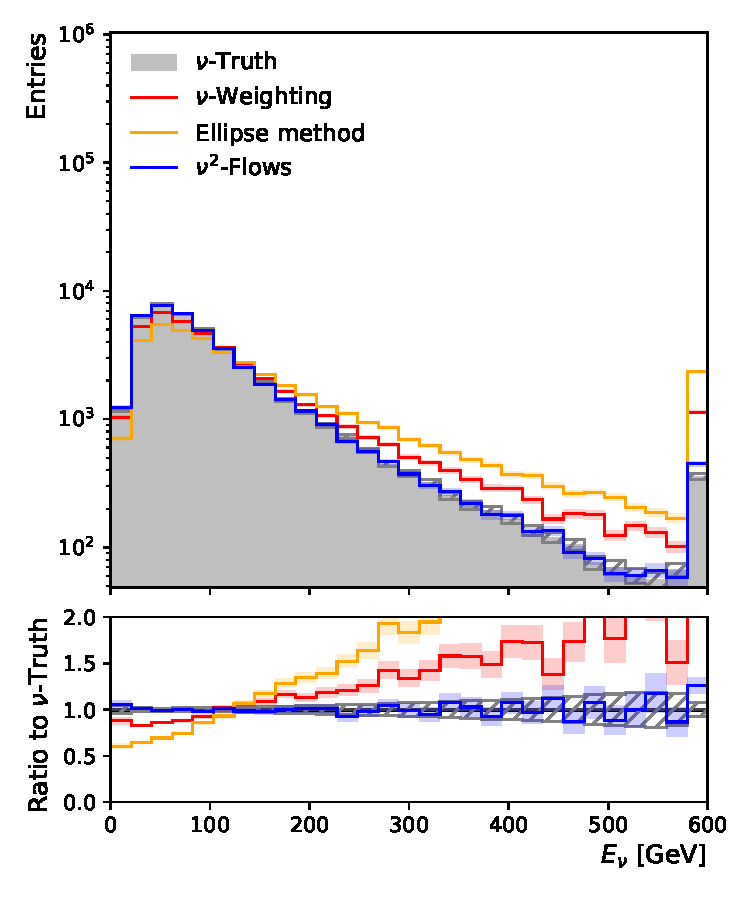
\includegraphics[width=0.32\textwidth]{Figures/neutrino_unfolding/nu_reco/nuanti_nu_E.pdf}
    \caption{The kinematics of the reconstructed (anti-)neutrinos for the three reconstruction methods and \vtruth (shaded grey). The shaded areas represent statistical uncertainties.}
    \label{fig:vvbarkinematics}
\end{figure}

\begin{figure}[htpb]
    \centering
    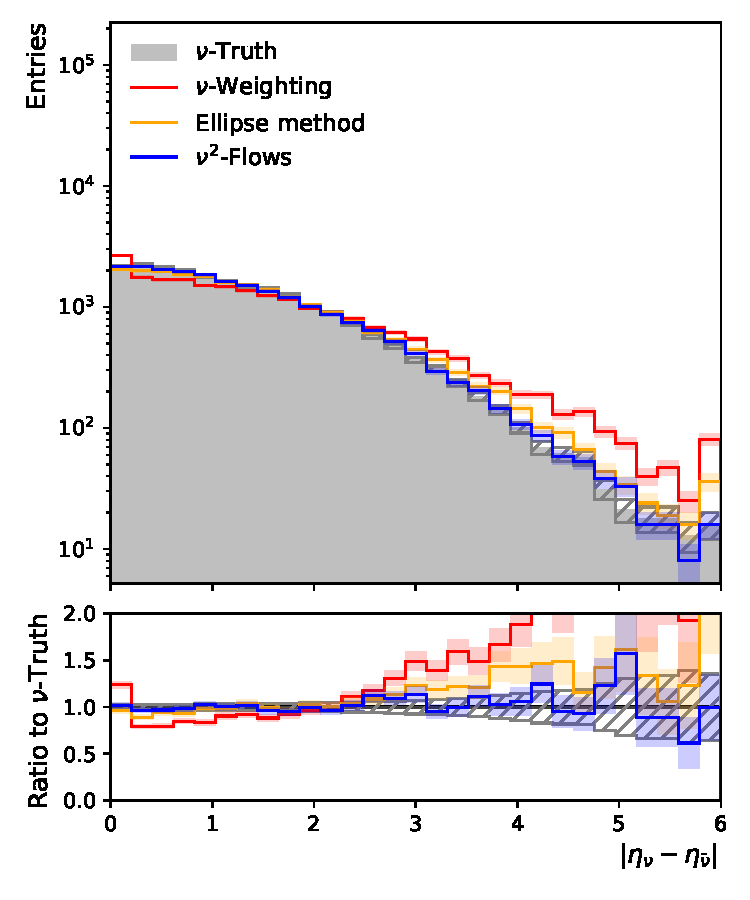
\includegraphics[width=0.32\textwidth]{Figures/neutrino_unfolding/nu_reco/nu_del_eta.pdf}
    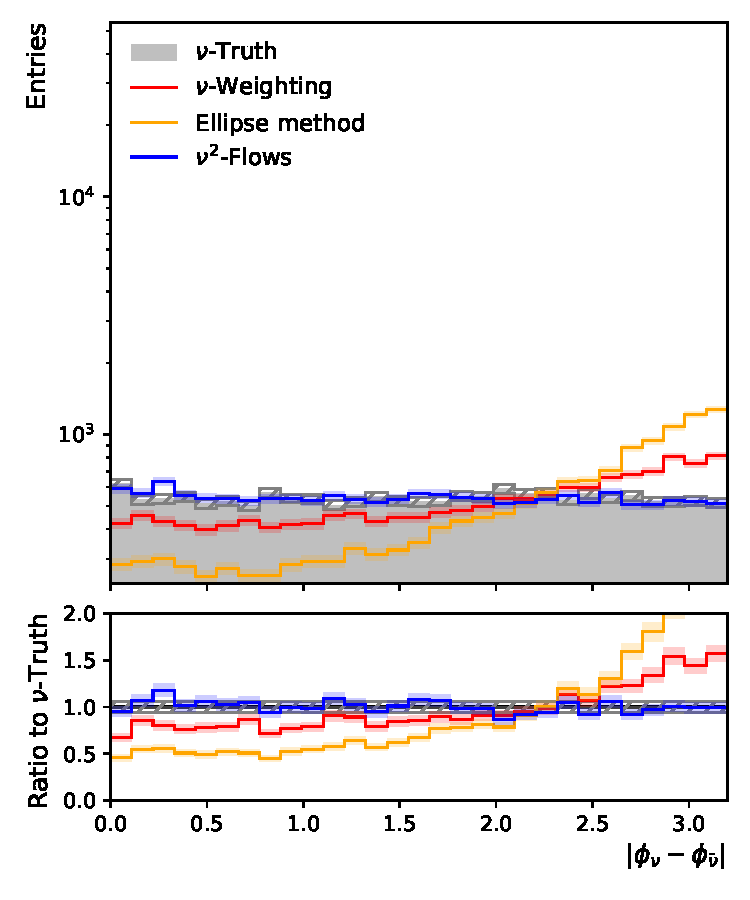
\includegraphics[width=0.32\textwidth]{Figures/neutrino_unfolding/nu_reco/nu_del_phi.pdf}
    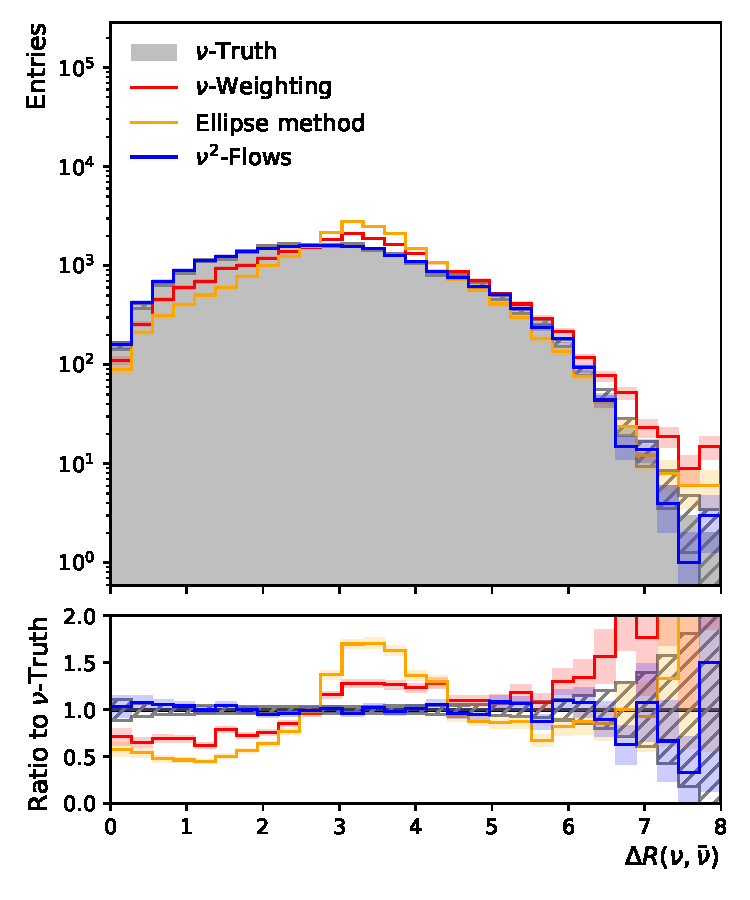
\includegraphics[width=0.32\textwidth]{Figures/neutrino_unfolding/nu_reco/nu_del_R.pdf}
    \caption{The angular separation in $\eta$ and $\phi$ between the reconstructed neutrino pair per event for the three reconstruction methods and \vtruth (shaded grey). The shaded areas represent statistical uncertainties.}
    \label{fig:vreco_delta}
\end{figure}

From the reconstructed neutrinos, it is possible to also reconstruct the \Wbosons, top quarks, and the full \ttbar system in the event.
\Cref{fig:Wtmasspt} shows the reconstructed invariant mass of the \Wboson and top quark using the perfect association of jets and leptons to the two top quarks.
The \vweight and \ellipse methods exhibit a strong bias towards the top quark and \Wboson masses as defined in \Cref{eq:mass_constraints}.
In contrast, \vvflows aligns with the underlying target distribution for the \Wboson mass and better captures the reconstructed top-quark mass distribution, albeit with a lower resolution than \vtruth.
The reconstructed top quark \pt is accurately reproduced with \vvflows and up to approximately 200~GeV by \vweight, whereas \ellipse tends to reconstruct top quarks with a harder \pt.

\begin{figure}[htbp]
    \centering
    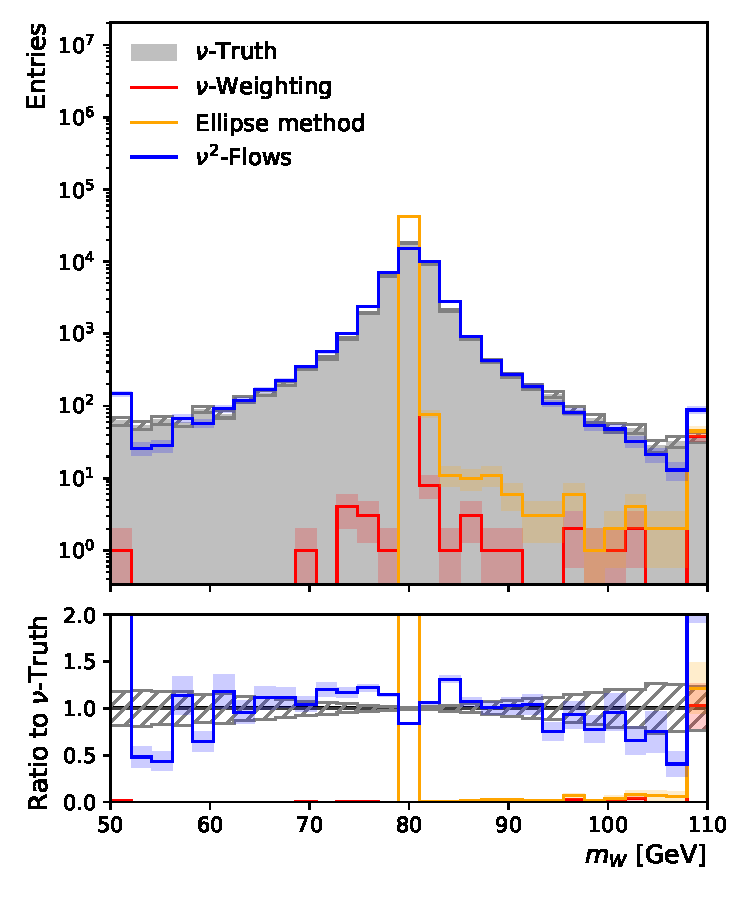
\includegraphics[width=0.32\textwidth]{Figures/neutrino_unfolding/ttbar_reco/W_plusW_minus_m.pdf}
    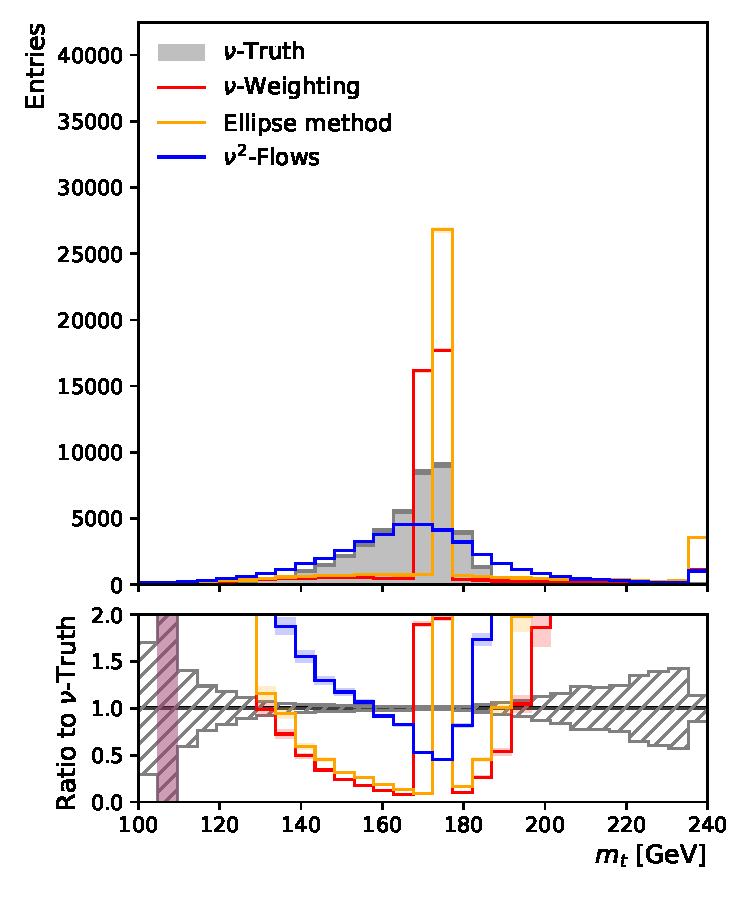
\includegraphics[width=0.32\textwidth]{Figures/neutrino_unfolding/ttbar_reco/topanti_top_m.pdf}
    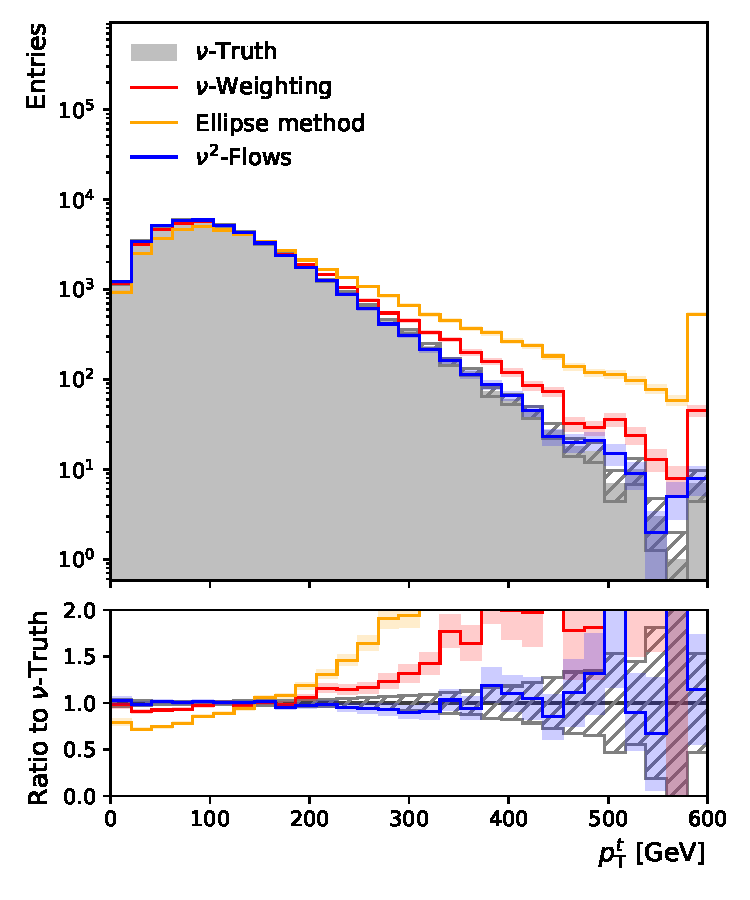
\includegraphics[width=0.32\textwidth]{Figures/neutrino_unfolding/ttbar_reco/topanti_top_pt.pdf}
    \caption{The reconstructed invariant mass of \Wbosons (left) and top quarks (middle), as well as the top quark \pt (right) when using the three neutrino reconstruction methods in comparison to \vtruth (shaded grey). The shaded areas represent statistical uncertainties.}
    \label{fig:Wtmasspt}
\end{figure}

In \Cref{fig:ttbar_kin}, the invariant mass, \pt, and rapidity of the reconstructed \ttbar system \ytt are shown.
Although \vvflows closely reproduces the kinematics of the \ttbar system, some discrepancies are observed at low \mttbar values.
The \pttt and \ytt distributions are well reconstructed with \vweight, but there is an overestimate in the tail of the \mttbar distribution.
In contrast, \ellipse shows poor modelling in both the \mttbar and \pttt distributions.

\begin{figure}[tbp]
    \centering
    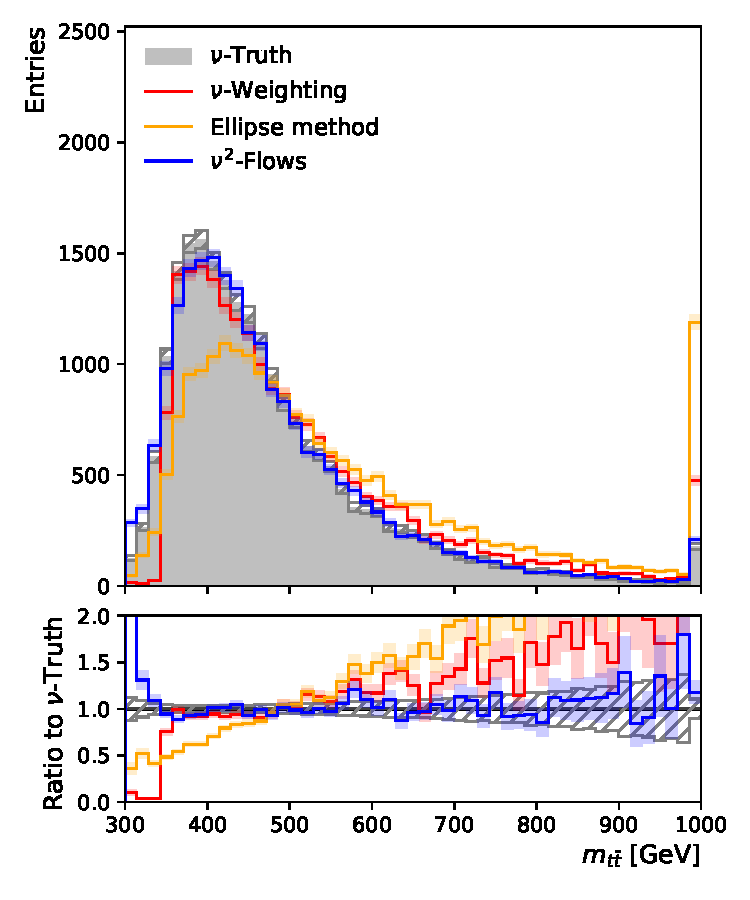
\includegraphics[width=0.32\textwidth]{Figures/neutrino_unfolding/ttbar_reco/ttbar_m.pdf}
    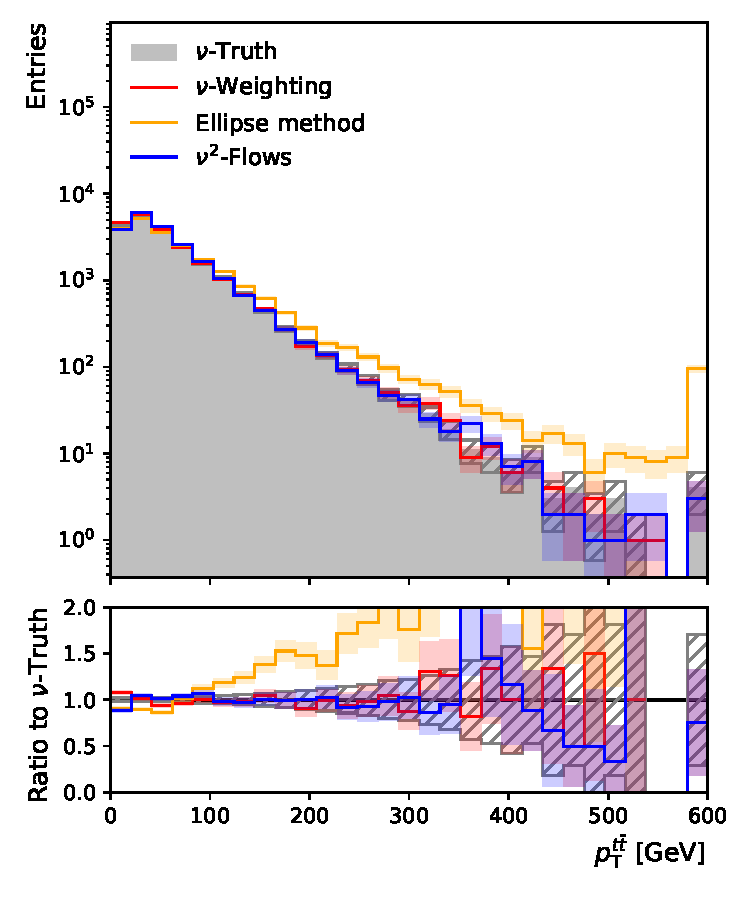
\includegraphics[width=0.32\textwidth]{Figures/neutrino_unfolding/ttbar_reco/ttbar_pt.pdf}
    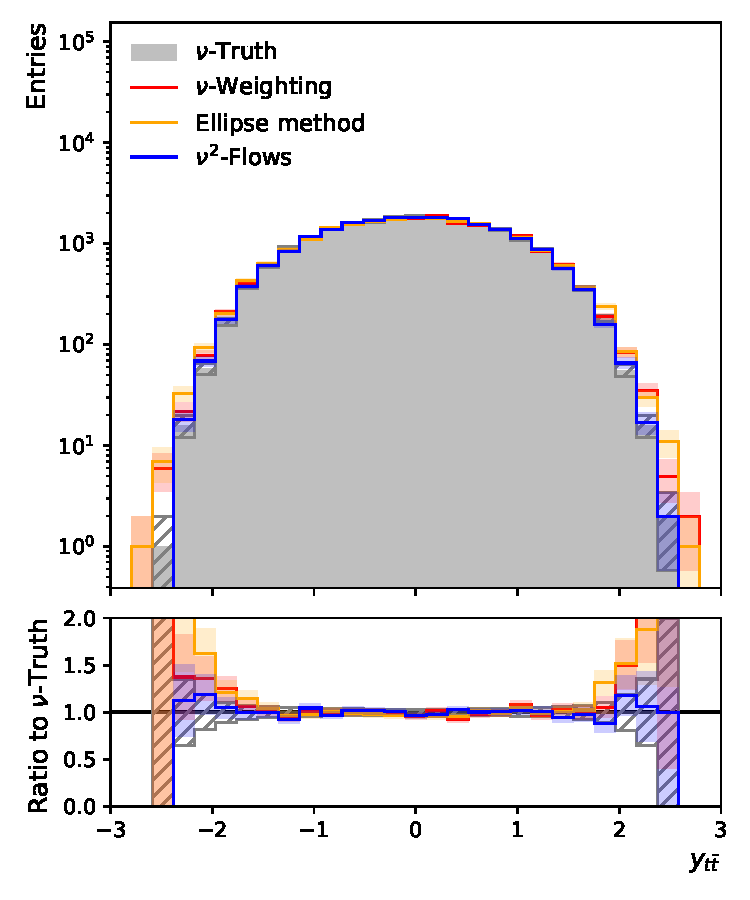
\includegraphics[width=0.32\textwidth]{Figures/neutrino_unfolding/ttbar_reco/ttbar_rapidity.pdf}
    \caption{The invariant mass, \pt, and rapidity of the reconstructed \ttbar system when using the three neutrino reconstruction methods in comparison to \vtruth (shaded grey). The shaded areas represent statistical uncertainties.}
    \label{fig:ttbar_kin}
\end{figure}

\subsubsection{Unfolding Analysis}

To evaluate the downstream impact of the improved neutrino reconstruction, we follow the unfolding analysis in Ref.~\cite{ATLAS:2016pbv}.
In this analysis, normalized differential cross-sections in the fiducial phase space region for specific \ttbar system observables are unfolded to the particle level.
These observables are shown in \Cref{tab:diff_observables}, including extra observables motivated by a similar study~\cite{CMS:2017iqf}, each depending on the neutrino kinematics.
In the reference analysis, the \vweight method is used to reconstruct the neutrinos, which is then used to reconstruct the observables, which are then unfolded using iterative Bayesian unfolding.
For our reimplementation, we compare this process using \vvflows, \vweight, \ellipse, and \vtruth to determine the neutrino kinematics.

Double differentiable unfolding is performed by initially binning the data in \mttbar, then in the observable of interest.
The correct jet and lepton associations for both top quarks are used to eliminate matching inefficiencies.
We perform the unfolding using the Singular Value Decomposition (SVD) method~\cite{SVDApproachData} with a regularization factor of 7, using the RooUnfold~\cite{ComparisonUnfoldingMethods} package.
The regularization factor was optimized for the \vtruth distributions for a reduced $\chi^2$ value closest in agreement with one for the four double differential distributions.
We do not make measurements of the cross-section in this work but instead focus on the statistical uncertainties of the unfolded distributions, which are compared to the optimal performance using \vtruth.

\begin{table}[htbp]
    \centering
    \caption{Kinematic observables of the reconstructed \ttbar system studied for an unfolding analysis in dilepton events and their bin edges.}
    \label{tab:diff_observables}
    \resizebox{\textwidth}{!}{
        \begin{tabular}{clll}
            \toprule
            Observable & Description                                  & Bin edges                               \\
            \midrule
            \mttbar    & Invariant mass of \ttbar system              & [0, 400, 500, 800, inf]     & GeV       \\
            \dphill    & Separation in $\phi$ between the two leptons & [0.0, 0.25, 0.5, 0.75, 1.0] & rad/$\pi$ \\
            \pttop     & Transverse momentum of the top quark         & [0, 75, 125, 175, inf]      & GeV       \\
            \pttt      & Transverse momentum of the \ttbar system     & [0, 70, 140, 200, inf]      & $\GeV$    \\
            \ytt       & Rapidity of the \ttbar system                & [-inf, -1.0, 0.0, 1.0, inf] &           \\
            \bottomrule
        \end{tabular}
    }
\end{table}

The response matrix for each neutrino reconstruction method is depicted in \cref{fig:unfold_dphill} for the two-dimensional binning in \mttbar and \dphill, and in \cref{fig:unfold_pttop} for \mttbar and \pttop.
Ideally, only the main diagonal would have entries, but due to inefficiencies in the reconstruction methods and detector resolution effects, off-diagonal elements are present.
Using \vvflows results in a more diagonal response matrix, as quantified by the trace fraction shown in each plot's top right corner.

While the trace fraction indicates method performance, off-diagonal elements still impact the unfolded distributions.
To assess this impact true impact, response matrices are inverted using SVD, and overall uncertainties for each bin at the parton level are calculated.
\Cref{fig:stat_gain_unfold_all} displays the relative statistical uncertainty for each method compared to \vtruth, also shown in \Cref{tab:all_unfolding}.
Uncertainties in the four double differential distributions are typically 1.5 to 2 times smaller with \vvflows compared to \vweight and up to four times smaller compared to \ellipse.

\begin{figure*}[htp]
    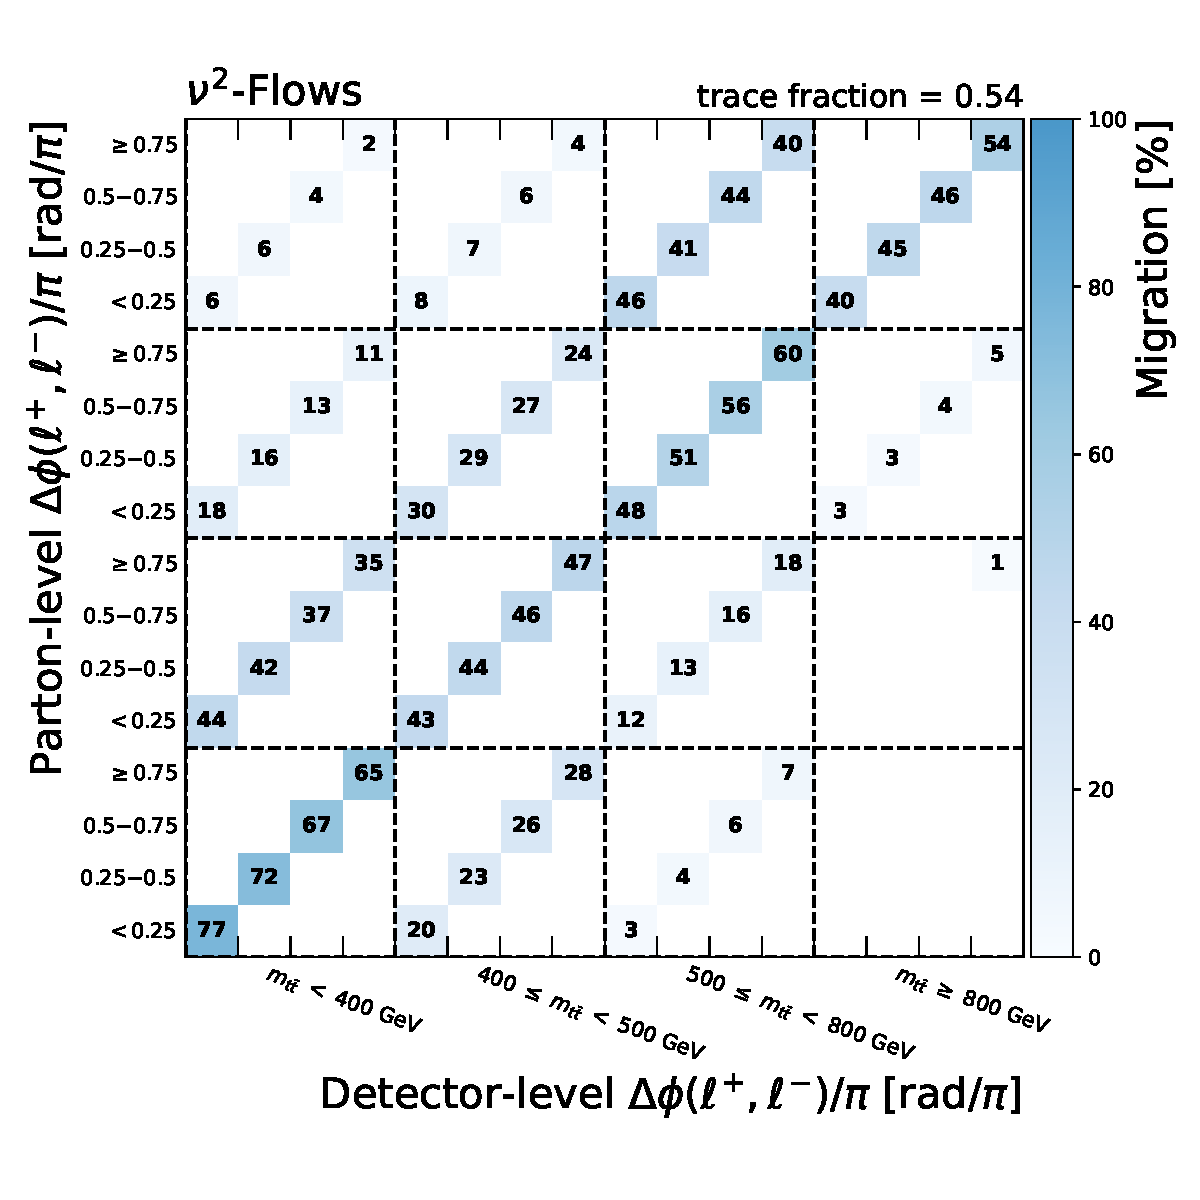
\includegraphics[width=0.32\textwidth]{Figures/neutrino_unfolding/unfolding/unfold_lep_delphi_transformer_encoder.pdf}
    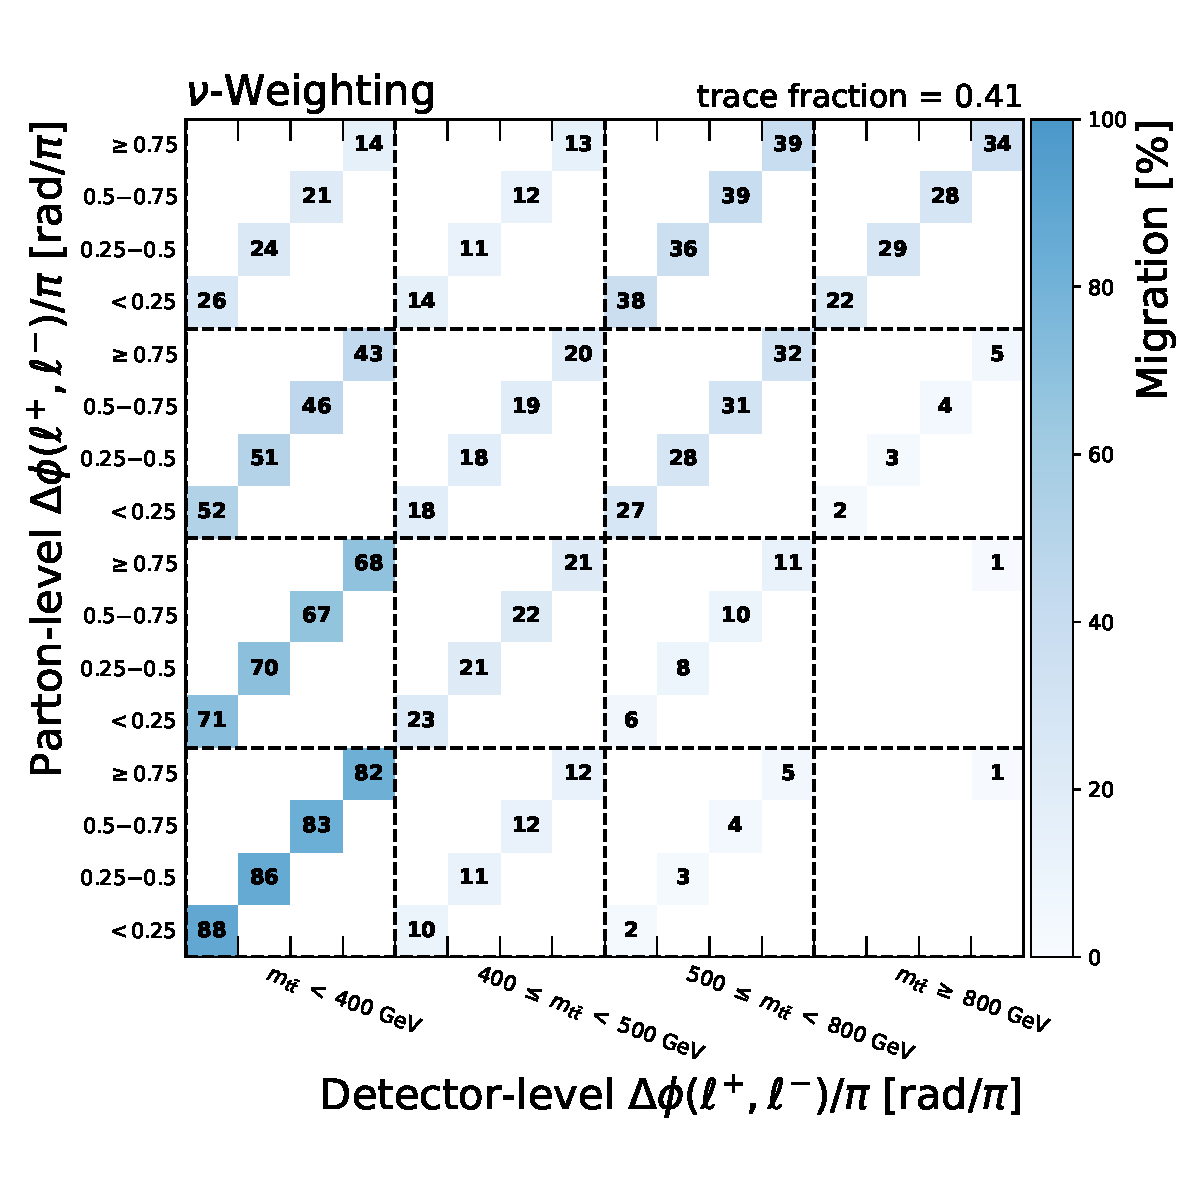
\includegraphics[width=0.32\textwidth]{Figures/neutrino_unfolding/unfolding/unfold_lep_delphi_nu_weighting.pdf}
    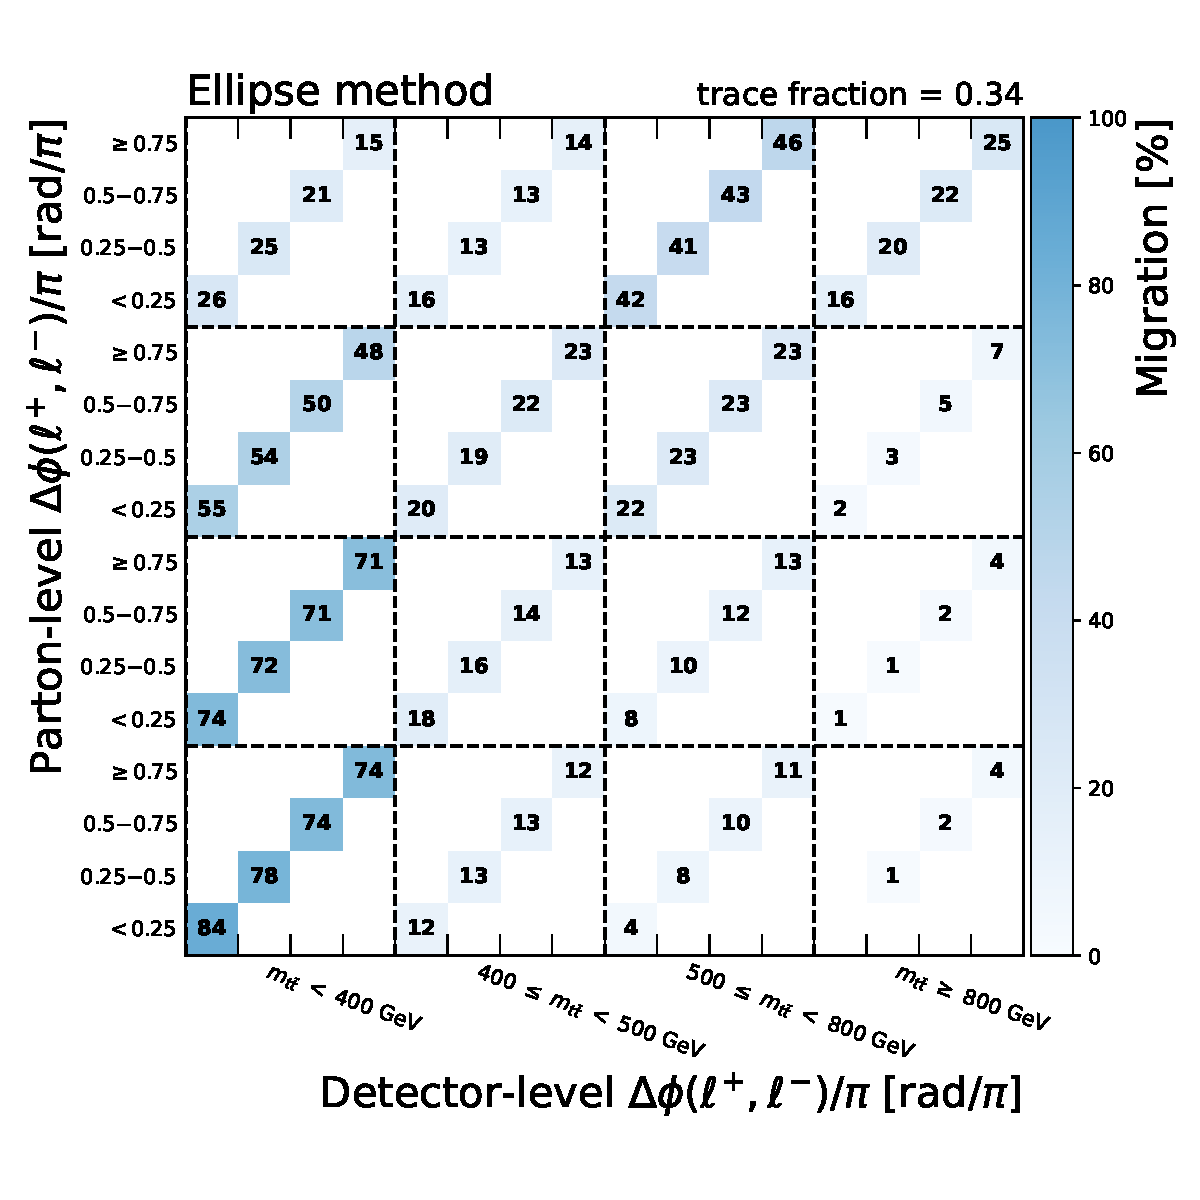
\includegraphics[width=0.32\textwidth]{Figures/neutrino_unfolding/unfolding/unfold_lep_delphi_nu_ellipse.pdf}
    \caption{Binned response matrices for the double differential measurement of \mttbar and \dphill when using each of the three methods for neutrino reconstruction. The binning is symmetric for both the parton and detector level observables, however the \mttbar bins are labelled on the $x$-axis with the \dphill bins labelled on the $y$-axis.
        The trace fraction is calculated for each method for a simple quantitative comparison and is 0.73 when using \vtruth.}
    \label{fig:unfold_dphill}
\end{figure*}

\begin{figure*}[htp]
    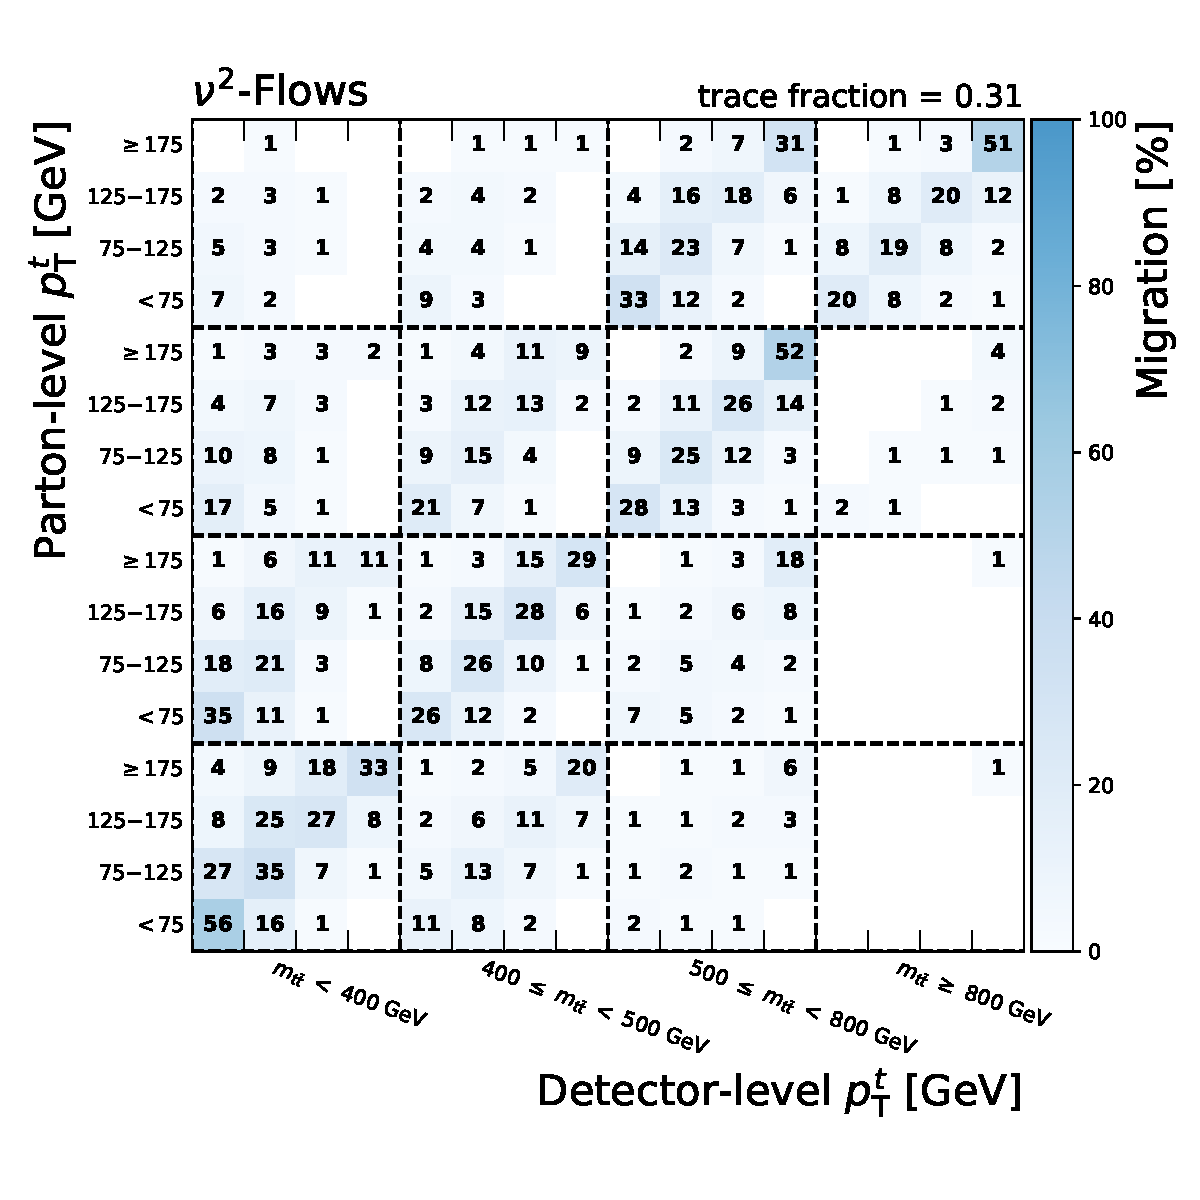
\includegraphics[width=0.32\textwidth]{Figures/neutrino_unfolding/unfolding/unfold_top_pt_transformer_encoder.pdf}
    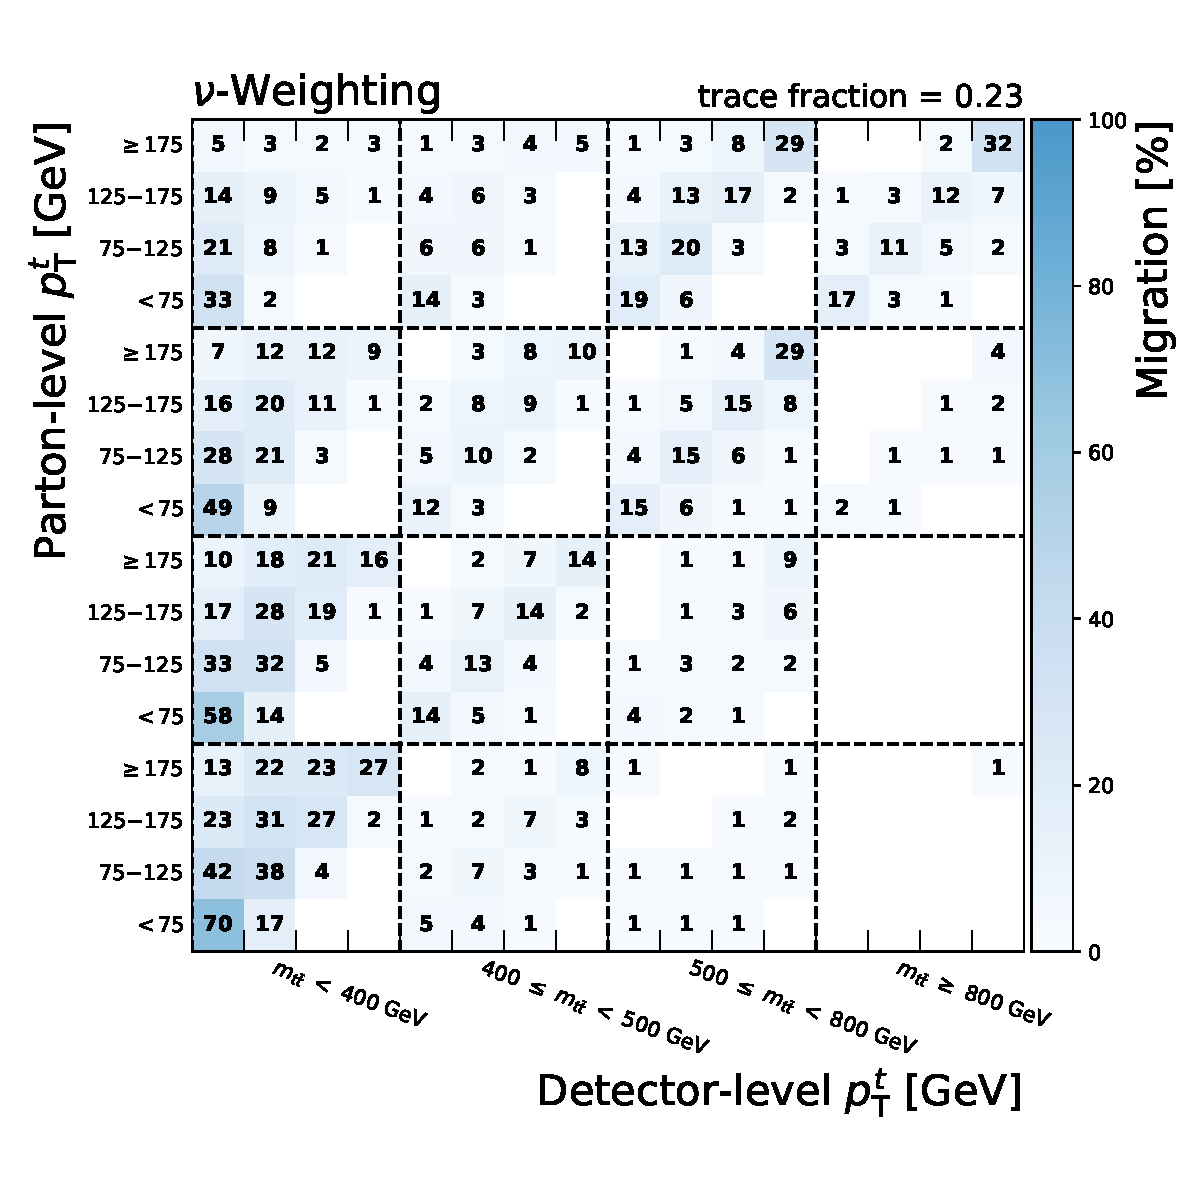
\includegraphics[width=0.32\textwidth]{Figures/neutrino_unfolding/unfolding/unfold_top_pt_nu_weighting.pdf}
    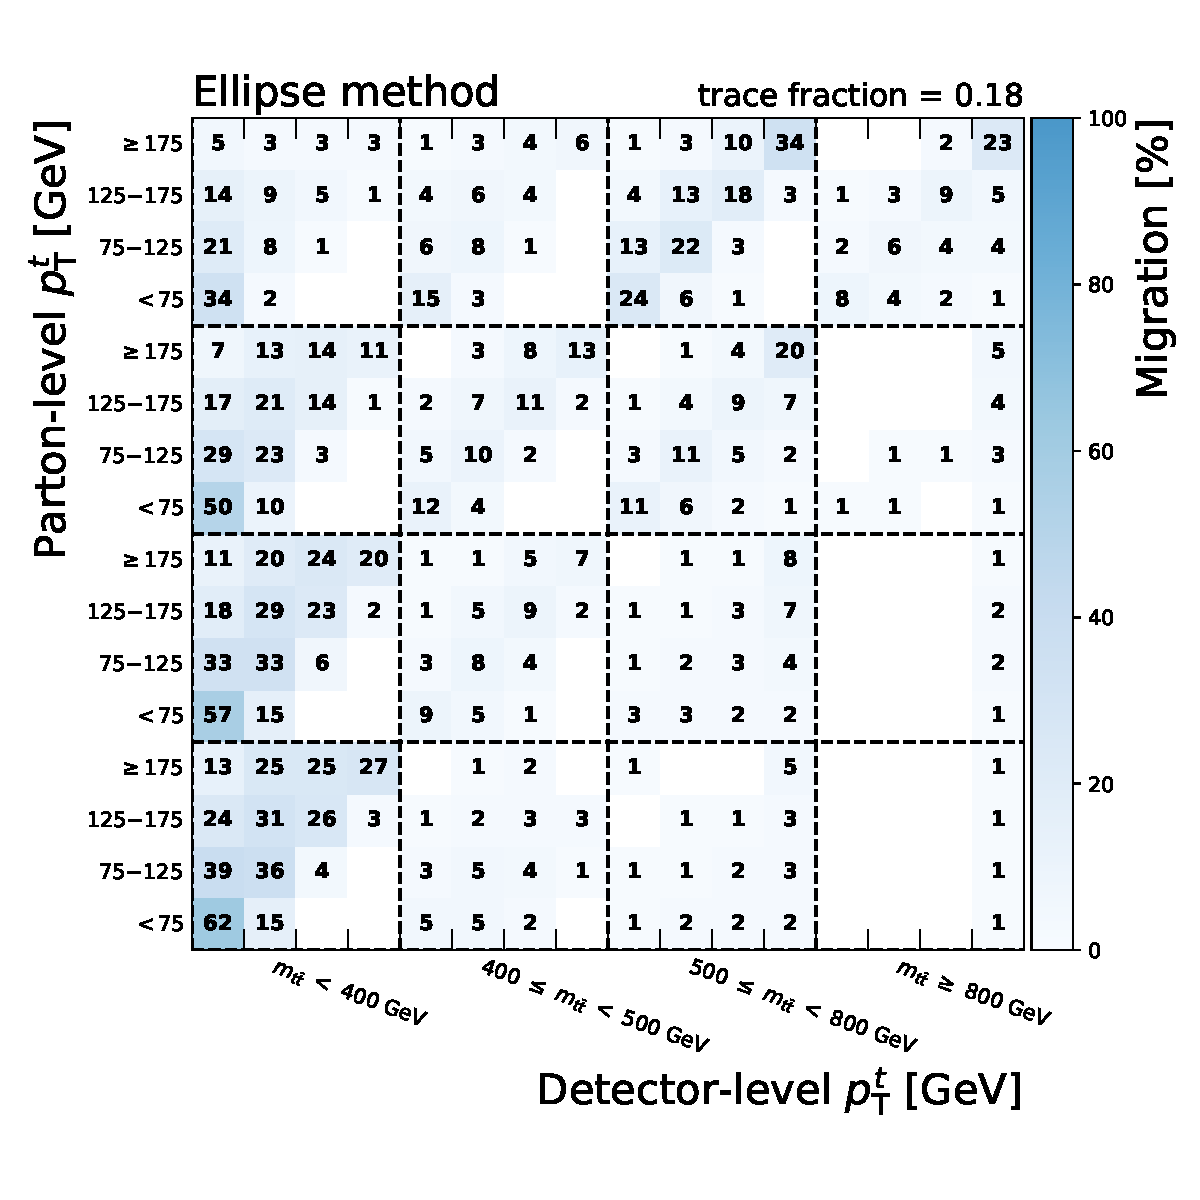
\includegraphics[width=0.32\textwidth]{Figures/neutrino_unfolding/unfolding/unfold_top_pt_nu_ellipse.pdf}
    \caption{Binned response matrices for the double differential measurement of \mttbar and \pttop when using each of the three methods for neutrino reconstruction. The binning is symmetric for both the parton and detector level observables, however the \mttbar bins are labelled on the $x$-axis with the \pttop bins labelled on the $y$-axis.
        The trace fraction is calculated for each method for a simple quantitative comparison and is 0.62 when using \vtruth.}
    \label{fig:unfold_pttop}
\end{figure*}

\begin{figure*}[htpb]
    \centering
    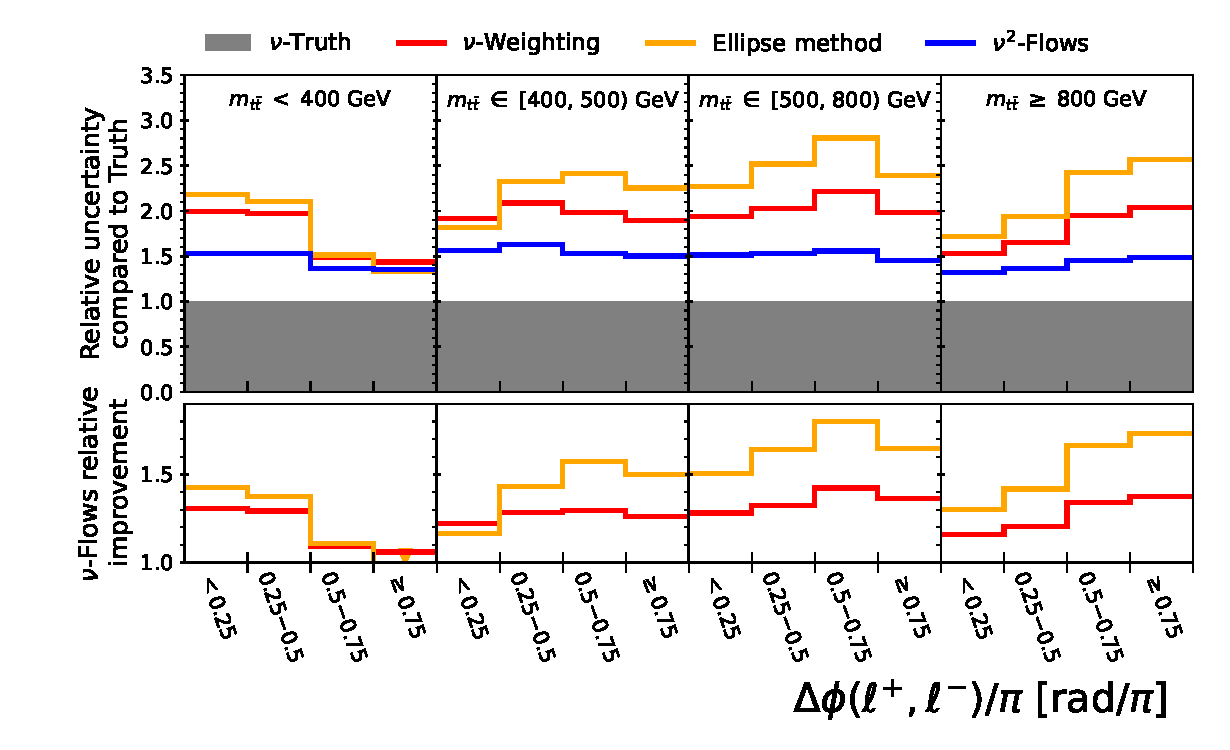
\includegraphics[width=0.48\textwidth]{Figures/neutrino_unfolding/unfolding/unfold_error_lep_del_phi_7.pdf}
    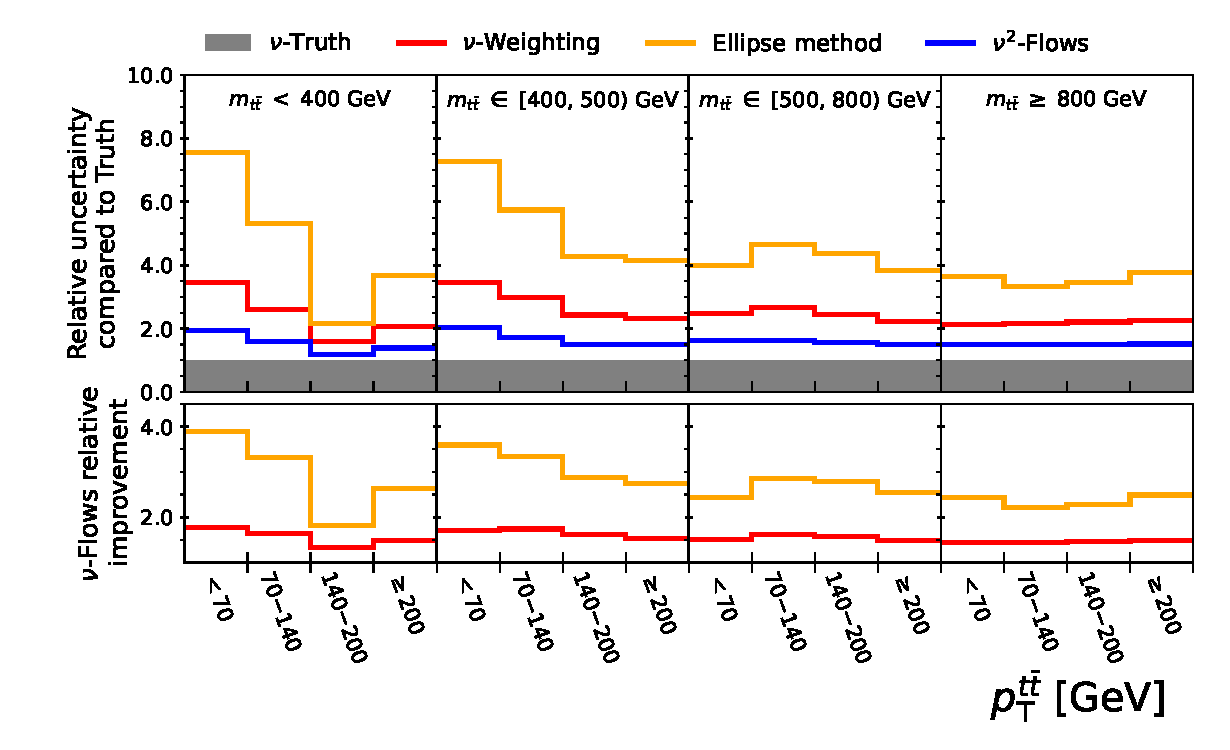
\includegraphics[width=0.48\textwidth]{Figures/neutrino_unfolding/unfolding/unfold_error_ttbar_pt_7.pdf} \\
    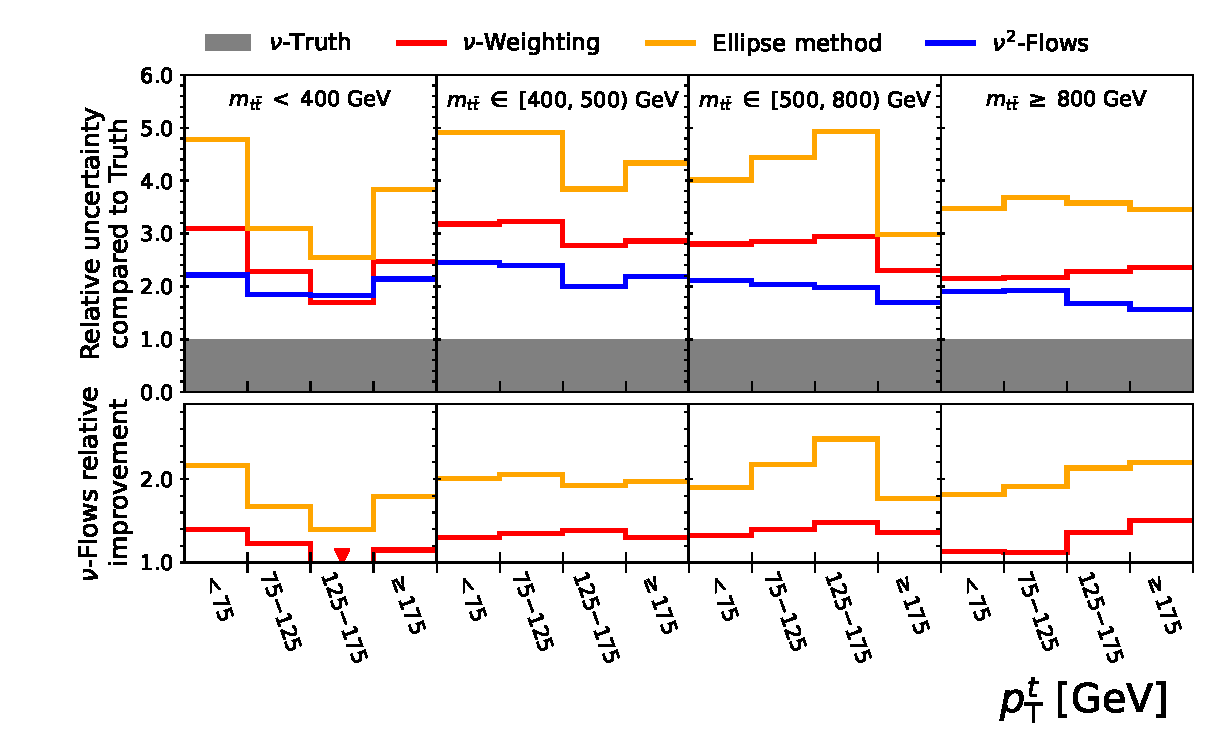
\includegraphics[width=0.48\textwidth]{Figures/neutrino_unfolding/unfolding/unfold_error_top_pt_7.pdf}
    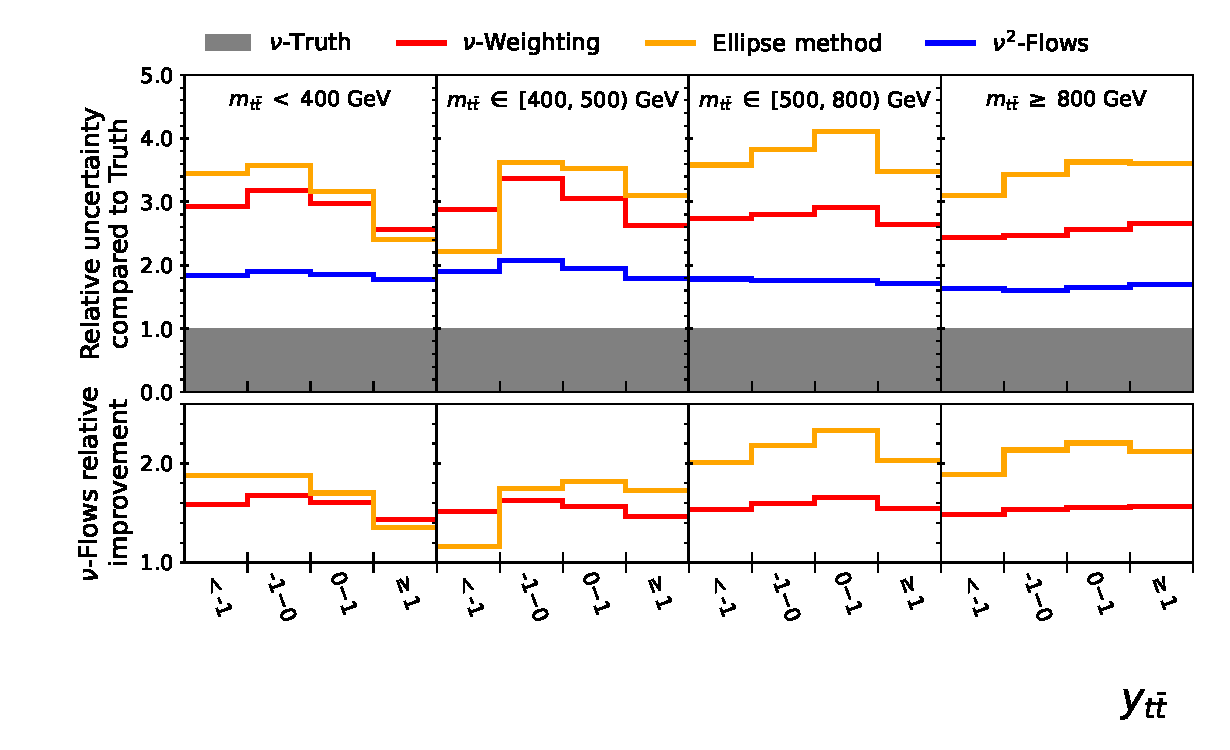
\includegraphics[width=0.48\textwidth]{Figures/neutrino_unfolding/unfolding/unfold_error_ttbar_rapidity_7.pdf}
    \caption{The relative statistical uncertainty in each unfolded bin of the two-dimensional distributions for \mttbar and \dphill (top left), \pttop (top right), \pttt (bottom left), and \ytt (bottom right).
        Comparing the three reconstruction methods with respect to \vtruth (upper pad), and the relative improvement of \vflows with respect to \vweight and \ellipse (lower pad).}
    \label{fig:stat_gain_unfold_all}
\end{figure*}

\subsubsection{Robustness to Training Sample}

Compared to standard analytical methods, \vflows is trained on MC simulated events.
This may result in the model learning sample-specific effects, and lead to suboptimal or even unusable performance when applied to different samples from other generators.
To evaluate this effect, \vvflows was trained using the alternative \ttbar dilepton sample (\vvflowsPy) and used to reconstruct the neutrinos for the nominal \ttbar sample.
We compare the reconstructed kinematic distributions as well as the unfolding performance.

Negligible differences are observed in the reconstructed neutrino kinematics, though the minor offsets can clearly be seen for the reconstructed \Wboson mass top quark invariant masseses.
For the double differential unfolding analysis, there is a slight change in the statistical uncertainty in each bin after unfolding, shown in \Cref{tab:all_unfolding}.
However, most of these changes are minor and the method still outperforms \vweight and \ellipse.

\begin{figure}[htbp]
    \centering
    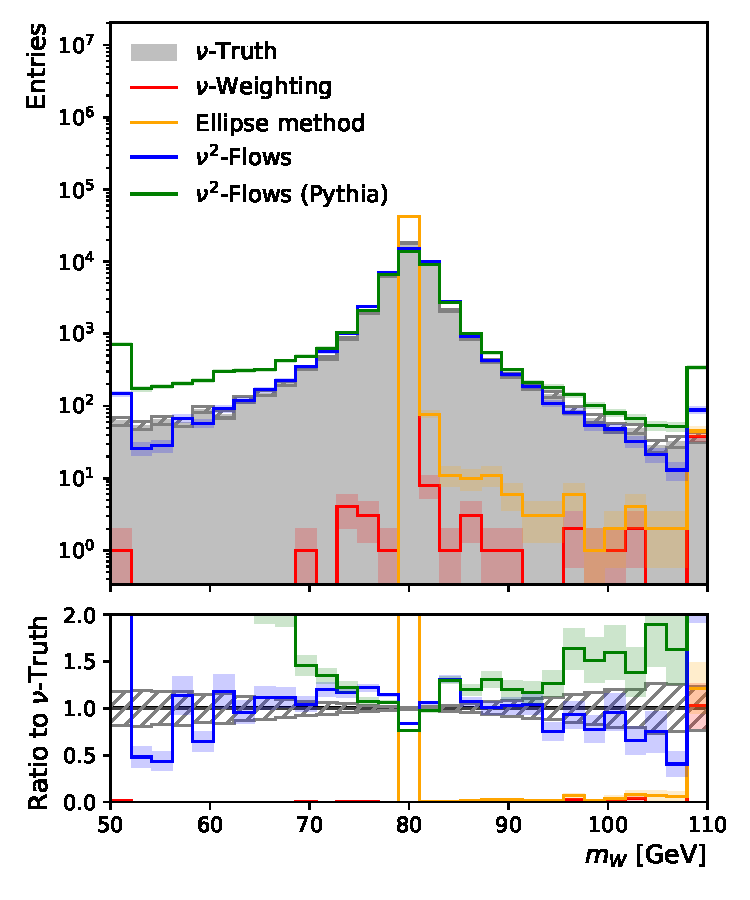
\includegraphics[width=0.32\textwidth]{Figures/neutrino_unfolding/pythia8/W_plusW_minus_m.pdf}
    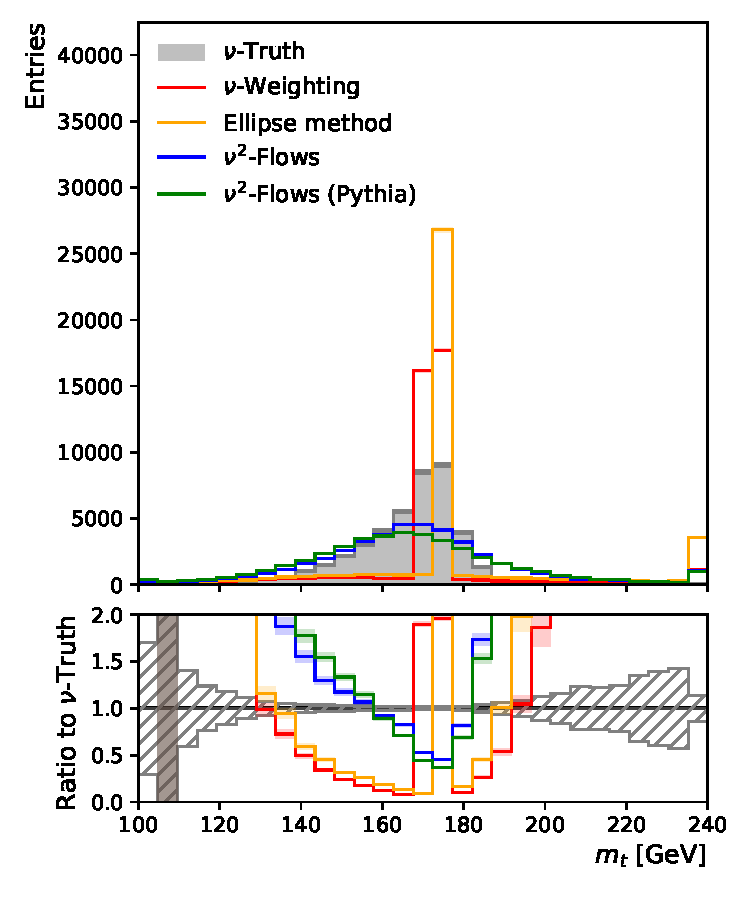
\includegraphics[width=0.32\textwidth]{Figures/neutrino_unfolding/pythia8/topanti_top_m.pdf}
    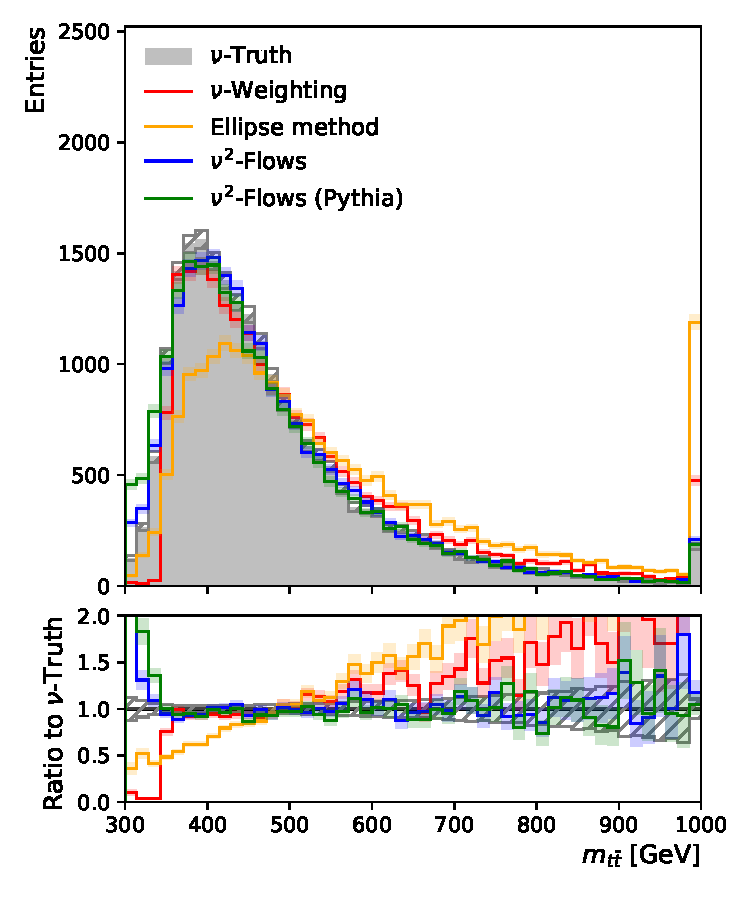
\includegraphics[width=0.32\textwidth]{Figures/neutrino_unfolding/pythia8/ttbar_m.pdf}
    \caption{
        The invariant masses of the reconstructed \Wboson, top quark, and \ttbar system when using \vvflows trained on the nominal or alternative sample, in comparison to the two baseline approaches and \vtruth (shaded grey).
    }
    \label{fig:pythiattbar}
\end{figure}

\begin{table}[thp]
    \centering
    \caption{Relative uncertainty in each bin of the respective unfolded double differential distributions for each neutrino reconstruction method with respect to the uncertainty when using \vtruth. The bins are ordered first by increasing \mttbar followed by the second variable, with vertical dividers indicating the bin edges in \mttbar. The method with the smallest relative increase in uncertainty in comparison to \vtruth is highlighted in bold.}
    \label{tab:app:rel_unfold_uncerts}
    \resizebox{\textwidth}{!}{
        \begin{tabular}{c c r r r r r | r r r r | r r r r | r r r r}
    \toprule
    \multicolumn{2}{c}{Observables} & Method & \multicolumn{16}{c}{Relative uncertainty to \vtruth (per bin)}\\
    \midrule

    \multirow{16}{*}{\mttbar} & \multirow{4}{*}{\ytt}
    & \vweight & 2.9 & 3.2 & 3.0 & 2.6 & 2.9 & 3.4 & 3.1 & 2.6 & 2.7 & 2.8 & 2.9 & 2.6 & 2.4 & 2.5 & 2.6 & 2.7\\
    & & \ellipse & 3.5 & 3.6 & 3.2 & 2.4 & 2.2 & 3.6 & 3.5 & 3.1 & 3.6 & 3.8 & 4.1 & 3.5 & 3.1 & 3.4 & 3.6 & 3.6\\
    & & \vvflows & \textbf{1.8} & \textbf{1.9} & \textbf{1.9} & \textbf{1.8} & \textbf{1.9} & \textbf{2.1} & \textbf{1.9} & \textbf{1.8} & \textbf{1.8} & \textbf{1.8} & \textbf{1.8} & \textbf{1.7} & \textbf{1.6} & \textbf{1.6} & \textbf{1.6} & \textbf{1.7}\\
    & & \vvflowsPy & 1.9 & \textbf{1.9} & \textbf{1.9} & \textbf{1.8} & \textbf{1.9} & \textbf{2.1} & 2.0 & \textbf{1.8} & \textbf{1.8} & \textbf{1.8} & \textbf{1.8} & \textbf{1.7} & 1.7 & \textbf{1.6} & 1.7 & 1.8\\

    \cmidrule{2-19}
    & \multirow{4}{*}{\pttt}
    & \vweight & 3.5 & 2.6 & 1.6 & 2.1 & 3.4 & 3.0 & 2.4 & 2.3 & 2.5 & 2.7 & 2.5 & 2.2 & 2.1 & 2.2 & 2.2 & 2.3\\
    & & \ellipse & 7.6 & 5.3 & 2.2 & 3.7 & 7.3 & 5.7 & 4.3 & 4.1 & 4.0 & 4.7 & 4.4 & 3.8 & 3.6 & 3.3 & 3.5 & 3.8\\
    & & \vvflows & \textbf{1.9} & \textbf{1.6} & \textbf{1.2} & \textbf{1.4} & \textbf{2.0} & \textbf{1.7} & \textbf{1.5} & \textbf{1.5} & \textbf{1.6} & \textbf{1.6} & \textbf{1.6} & \textbf{1.5} & \textbf{1.5} & \textbf{1.5} & \textbf{1.5} & \textbf{1.5}\\
    & & \vvflowsPy & 2.0 & \textbf{1.6} & \textbf{1.2} & \textbf{1.4} & \textbf{2.0} & \textbf{1.7} & \textbf{1.5} & \textbf{1.5} & 1.7 & \textbf{1.6} & \textbf{1.6} & \textbf{1.5} & \textbf{1.5} & \textbf{1.5} & \textbf{1.5} & \textbf{1.5}\\

    \cmidrule{2-19}
    & \multirow{4}{*}{\pttop}
    & \vweight & 3.1 & 2.3 & \textbf{1.7} & 2.5 & 3.2 & 3.2 & 2.8 & 2.9 & 2.8 & 2.9 & 2.9 & 2.3 & 2.2 & 2.2 & 2.3 & 2.4\\
    & & \ellipse & 4.8 & 3.1 & 2.5 & 3.8 & 4.9 & 4.9 & 3.8 & 4.3 & 4.0 & 4.4 & 4.9 & 3.0 & 3.5 & 3.7 & 3.6 & 3.4\\
    & & \vvflows & \textbf{2.2} & \textbf{1.9} & 1.8 & \textbf{2.1} & \textbf{2.5} & \textbf{2.4} & \textbf{2.0} & \textbf{2.2} & \textbf{2.1} & \textbf{2.0} & \textbf{2.0} & \textbf{1.7} & \textbf{1.9} & \textbf{1.9} & \textbf{1.7} & \textbf{1.6}\\
    & & \vvflowsPy & 2.3 & \textbf{1.9} & 1.9 & 2.2 & \textbf{2.5} & \textbf{2.4} & \textbf{2.0} & 2.3 & 2.2 & 2.1 & \textbf{2.0} & \textbf{1.7} & 2.0 & 2.0 & \textbf{1.7} & \textbf{1.6}\\

    \cmidrule{2-19}
    & \multirow{4}{*}{\dphill}
    & \vweight & 2.0 & 2.0 & 1.5 & 1.4 & 1.9 & 2.1 & 2.0 & 1.9 & 1.9 & 2.0 & 2.2 & 2.0 & 1.5 & 1.6 & 1.9 & 2.0\\
    & & \ellipse & 2.2 & 2.1 & 1.5 & \textbf{1.3} & 1.8 & 2.3 & 2.4 & 2.3 & 2.3 & 2.5 & 2.8 & 2.4 & 1.7 & 1.9 & 2.4 & 2.6\\
    & & \vvflows & \textbf{1.5} & \textbf{1.5} & \textbf{1.4} & 1.4 & \textbf{1.6} & \textbf{1.6} & \textbf{1.5} & \textbf{1.5} & \textbf{1.5} & \textbf{1.5} & \textbf{1.6} & \textbf{1.5} & \textbf{1.3} & \textbf{1.4} & \textbf{1.5} & \textbf{1.5}\\
    & & \vvflowsPy & \textbf{1.5} & \textbf{1.5} & \textbf{1.4} & 1.4 & \textbf{1.6} & \textbf{1.6} & \textbf{1.5} & \textbf{1.5} & \textbf{1.5} & \textbf{1.5} & \textbf{1.6} & 1.5 & \textbf{1.3} & \textbf{1.4} & \textbf{1.5} & \textbf{1.5}\\

    \bottomrule
\end{tabular}

    }
\end{table}

As an additional robustness test, we evaluate how \vvflows compares to \vweight and \ellipse in reconstructing \ttbar events simulated with extra ISR.
This sample consists of 280,000 events and is identical to the nominal sample, except for notable differences in jet multiplicity distributions and the underlying kinematics of the top-quark and \ttbar pair.
The distribution of \pttt, in particular, is significantly harder due to the recoil from the extra ISR.
\Cref{fig:extraISRttbar} shows the reconstructed distributions for the three approaches.
As before, \vvflows exhibits very good agreement across the majority of the kinematic phase space, despite having been optimised for a different sample.

\begin{figure}[htbp]
    \centering
    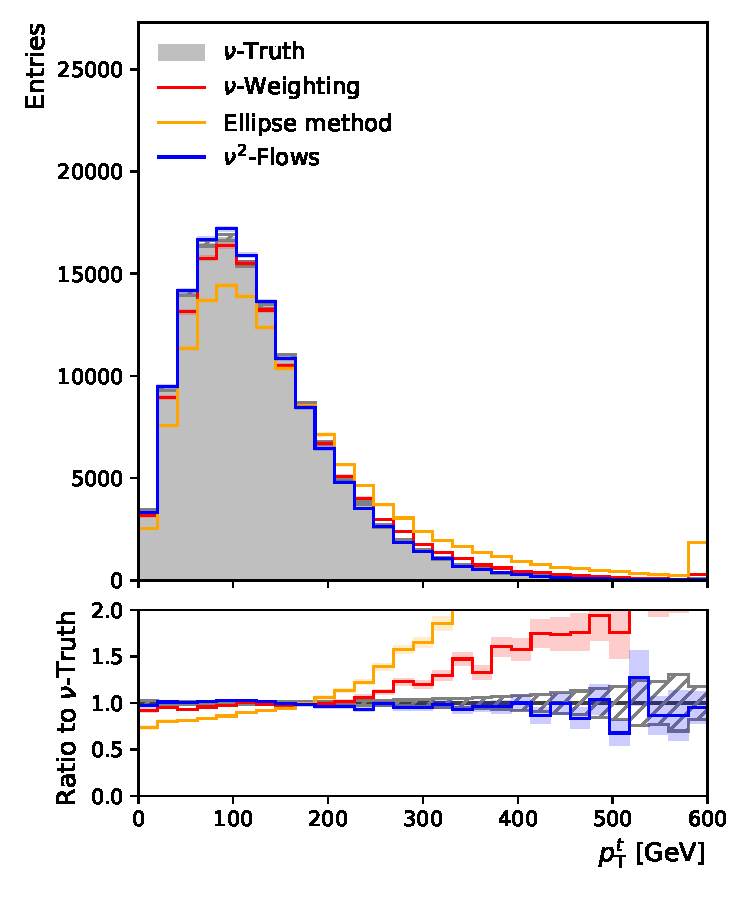
\includegraphics[width=0.32\textwidth]{Figures/neutrino_unfolding/extraISR/topanti_top_pt.pdf}
    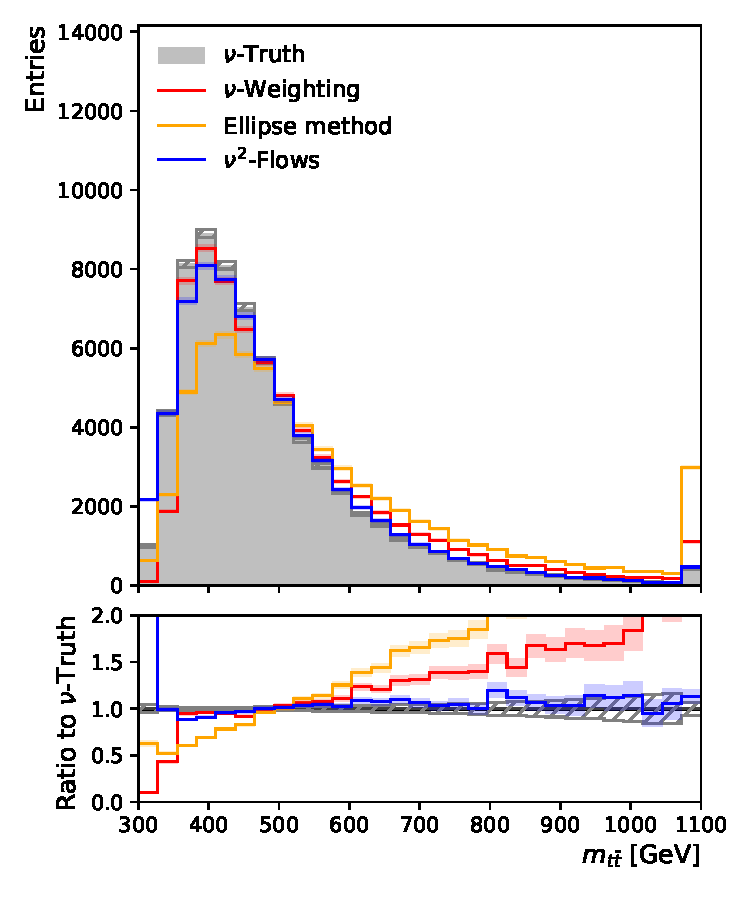
\includegraphics[width=0.32\textwidth]{Figures/neutrino_unfolding/extraISR/ttbar_m.pdf}
    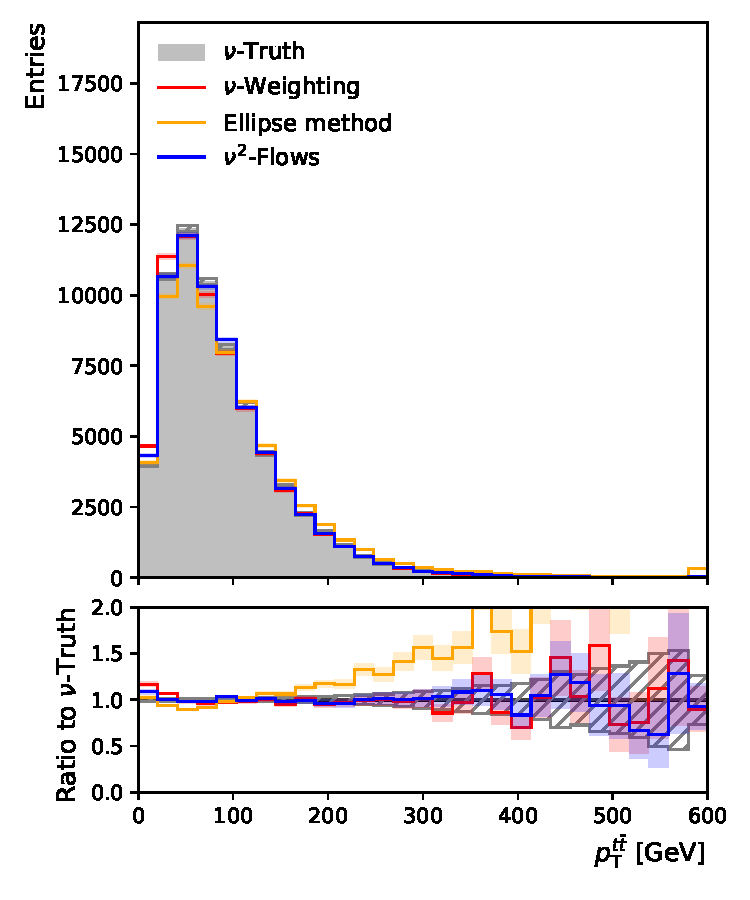
\includegraphics[width=0.32\textwidth]{Figures/neutrino_unfolding/extraISR/ttbar_pt.pdf}
    \caption{The reconstructed top quark \pt, and the invariant mass and \pt of the reconstructed \ttbar system for an independent sample with additional initial state radiation when using \vvflows trained on the nominal sample in comparison to the two baseline approaches and \vtruth (shaded grey).
    }
    \label{fig:extraISRttbar}
\end{figure}

\subsubsection{Sensitivity to Top Mass}

In contrast to \vweight and \ellipse, which both assume specific values for the top quark mass in the neutrino reconstruction \vvflows only implicitly learns this relation from the training data.
To test whether \vvflows has sensitivity to the underlying top quark mass, we use the default \vvflows model in a data sample where the generator top quark mass has been changed to either 171~GeV or 175~GeV.
These samples each have 160,000 events and are otherwise the same as the nominal.

The top quark mass is reconstructed using the lepton, $b$-jet, and neutrino.
A mass shift in the generated top quark mass should be reflected in the distributions of both the lepton-$b$ jet mass ($m_{b\ell}$) and the lepton-$b$-jet-neutrino mass ($m_t$).
We compare these two distributions to determine if the mass shift is more pronounced in $m_{b\ell\nu}$, indicating the neutrino's significant contribution to the reconstruction.

The distributions are shown in \cref{fig:top_mass_reco}.
Despite training purely on events with the nominal top quark mass, the reconstructed distribution using \vvflows is sensitive to the difference in truth $m_t$.
The separation between the three templates is similar to using $m_{b\ell}$, however for \vvflows the difference is more prominent in the bulk of the distribution.
This sensitivity could be improved by training \vvflows on samples with a range of values for $m_t$.
Another benefit of \vvflows is also demonstrated, with a smoother template constructed by sampling multiple neutrino solutions for each event.

\begin{figure*}[hbtp]
    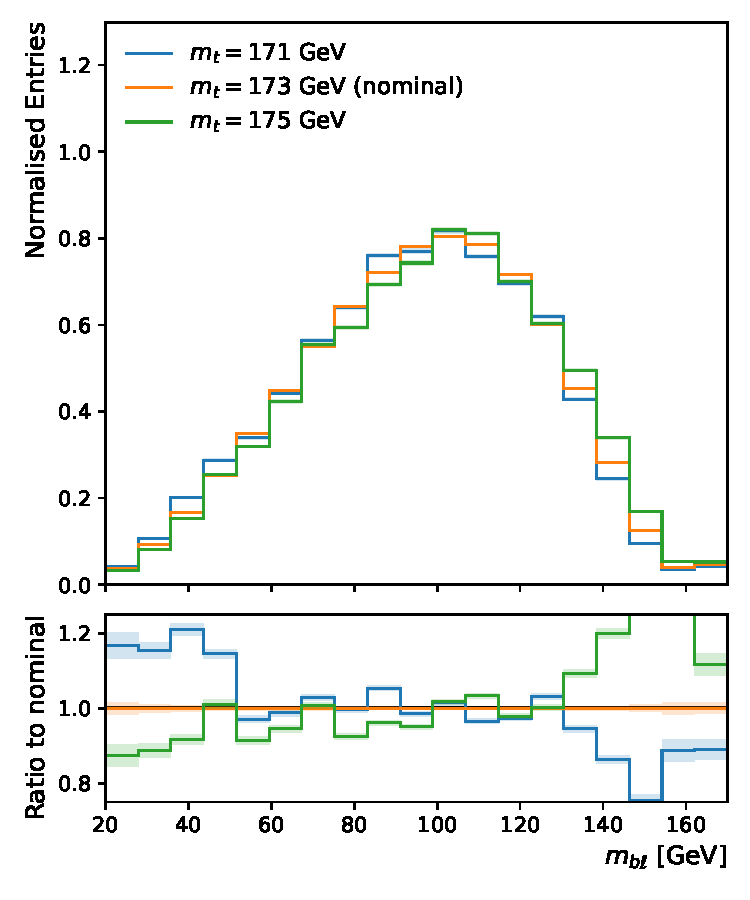
\includegraphics[width=0.32\textwidth]{Figures/neutrino_unfolding/mass_shift/both_bl_mass.pdf}
    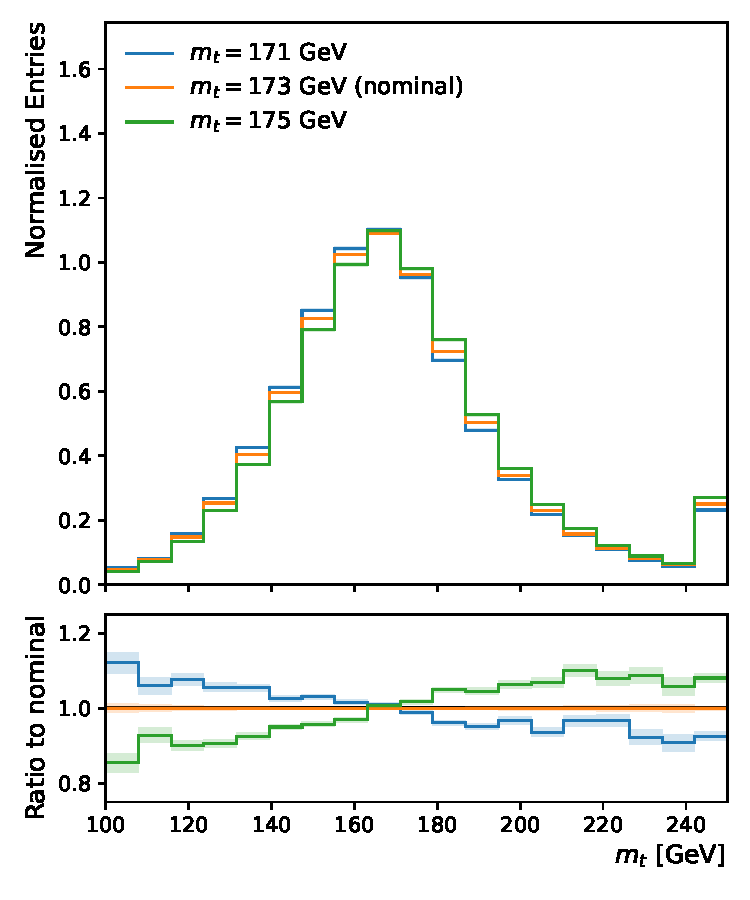
\includegraphics[width=0.32\textwidth]{Figures/neutrino_unfolding/mass_shift/both_top_mass_1.pdf}
    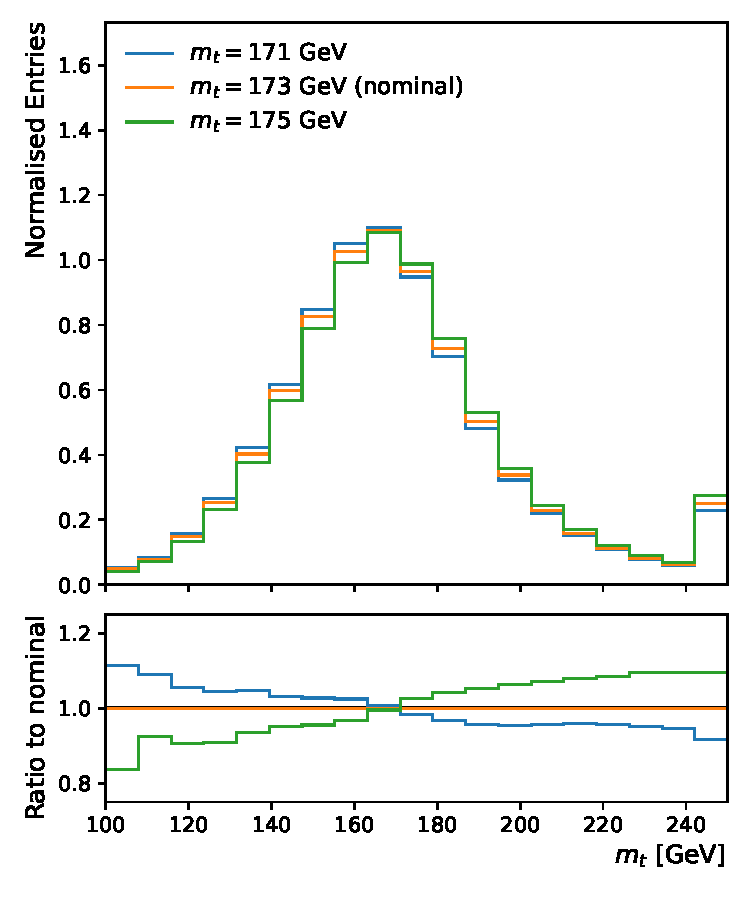
\includegraphics[width=0.32\textwidth]{Figures/neutrino_unfolding/mass_shift/both_top_mass_256.pdf}
    \caption{The reconstructed top quark mass using just from the lepton and $b$-quark from the top quark decay ($m_{b\ell}$, left), the full invariant mass using \vvflows to reconstruct the neutrinos from the top quarks ($m_t$, middle), and a smoothed template for $m_t$ obtained by sampling 256 solutions for each event with \vvflows (right).}
    \label{fig:top_mass_reco}
\end{figure*}

\section{Discussion and Future Work}

In conclusion, this chapter presents a comprehensive study of applying deep generative models, specifically normalizing flows, to the problem of neutrino unfolding in particle physics.
The proposed \vvflows method demonstrates significant improvements over traditional analytical techniques, such as the $m_W$ constraint for the single-neutrino case and \vweight and \ellipse methods for the two-neutrino case.
\vvflows can reconstruct individual neutrinos without enforcing strong constraints on reconstructed particle masses to find solutions in an under-constrained system, thus avoiding the biases that come with the other analytical methods.

The results show that \vvflows enhances the reconstruction of individual neutrino kinematics and improves the overall event reconstruction, leading to more accurate measurements of key observables in top quark physics.
These improvements can increase the sensitivity of the measurement of top quark spin correlation and entanglement at the LHC.
Furthermore, in contrast to other approaches, \vvflows has solutions for all events and the fast single event inference below 75~ms on a single computing core.

Future work includes extending this approach to final states with more than two neutrinos and training on a wide range of top quark masses for direct top quark mass measurements.

We could also investigate using the model as an event filter.
As each sample is associated with a probability from the transformation under the normalizing flow, this could also provide opportunities for separating \ttbar events from background processes, similar to the weight in \vweight.

Finally, while we have not noticed any significant shortcomings in the flow model's expressivity, a diffusion model could possibly achieve improved results.
One of the reasons for this is that the same model could be applied to final states with varying numbers of neutrinos using a denoising transformer encoder as used in \Cref{ch:jet_generation}.
